\pdfoutput=1
\documentclass[11pt]{article}
\usepackage[margin=1in]{geometry}
\usepackage[T1]{fontenc}
\usepackage[utf8]{inputenc}
\usepackage{lmodern}
\usepackage{microtype}
\usepackage{setspace}
\singlespacing
\usepackage{amsmath,amssymb}
\usepackage{graphicx}
\usepackage{booktabs}
\usepackage{tabularx}
\usepackage{longtable}
\usepackage{array}
\usepackage{caption}
\usepackage{subcaption}
\usepackage{tikz}
\usetikzlibrary{arrows.meta,positioning}
\usepackage[authoryear,round]{natbib}
\usepackage{url}
\usepackage{hyperref}
\captionsetup{font=small,labelfont=bf}
\captionsetup[subfigure]{font=footnotesize, justification=centering}
\hypersetup{colorlinks=true, linkcolor=black, citecolor=black, urlcolor=black,
  pdftitle={Constraint-Aware Traffic Intervention Visualization Using Multi-Label Road-Marking Recognition},
  pdfauthor={Farooq M. Anwar},
  pdfkeywords={multi-label classification; road markings; traffic congestion; decision support; constraint handling; reproducibility}}
\setlength{\emergencystretch}{3em}
\renewcommand{\arraystretch}{1.15}
\newcolumntype{Y}{>{\raggedright\arraybackslash}X}
\newcolumntype{P}[1]{>{\raggedright\arraybackslash}p{#1}}

\title{Constraint-Aware Traffic Intervention Visualization Using Multi-Label Road-Marking Recognition: Design, Audit, Correction, and Cross-Validated Evaluation of a Proof-of-Concept System}
\author{Farooq M. Anwar\\\small Independent Researcher}
\date{Preprint, October 2026}

\begin{document}
\maketitle

\begin{abstract}
I built a desktop prototype that recognizes road markings in aerial images, scores congestion from a roadway survey, filters a library of 30 interventions against user restrictions, and draws schematic overlays on the image. It was developed with 76 annotated map screenshots from Georgia, USA. This paper audits the 2025 development archive, corrects what the audit found, and evaluates the corrected recognition component. Twelve archived CNN training logs show validation AUC of 0.855--0.870 with 16 classes and 0.948--0.961 with 20 classes, but the label scheme changed between the two and validation used only 16 images, so the rise cannot be credited to better recognition. Re-running the archived decision code showed that only nine of 48 displayed restrictions were enforced (one of those never fired) and that detected markings had no effect on recommendations. I fixed these defects and evaluated the revised five-class EfficientNetV2S pipeline with repeated 5-fold stratified cross-validation, bootstrap confidence intervals, and baselines. The trained head reached a macro AUC of 0.684 (95\% CI 0.63--0.73), significantly below a logistic-regression probe on the same frozen features (0.738). Double Solid Yellow Line was indistinguishable from chance. At the fixed 0.35 threshold, recall was about 1.0 and precision sat near class prevalence, so thresholded outputs carried no information. The prototype does not establish calibrated recognition, congestion reduction, or safe roadway designs.
\end{abstract}

\noindent\textbf{Keywords:} multi-label classification; road markings; traffic congestion; decision support; constraint handling; reproducibility; small-data evaluation

\section{Introduction}
Whether a roadway intervention makes sense depends on the site. A measure that looks reasonable in a generic list may fail because there is no room for it, because of the intersection form, because of pedestrian or bicycle activity, or because of cost, policy, or an explicit prohibition. Visual tools can make alternatives easier to compare, but a convincing picture is not evidence. A decision-support system has to keep observed evidence, user assumptions, model outputs, and design judgment apart, and it has to show whether a stated restriction actually changes the recommendations.

This paper examines a desktop research prototype I built to explore that problem. The image component treats road-marking recognition as a multi-label task, since arrows, stop lines, and lane lines share scenes. The decision component computes an additive congestion index from a structured roadway survey, filters a library of 30 physical, operational, and policy interventions against user restrictions, and ranks what remains using subjective impact, safety, and cost values. OpenCV and Pillow routines then draw schematic interventions on a road image. The project started as a look at peak-hour traffic near a school campus, but the surviving records support no site-specific findings, so the paper is about the artifact and the limits of its evidence.

The development archive is messy. It holds changing class lists, duplicate logs, stale comments, and outputs from different software versions. Describing the latest architecture as if its performance had been measured would overstate the evidence, and throwing out the earlier runs would erase the implementation history. The study therefore has two parts. Part A is a retrospective audit of the 2025 archive that ties each claim to code, a complete training log, a deterministic check, or a qualitative output, and says which claims the archive cannot support. Part B, carried out in October 2026, corrects the defects the audit exposed and evaluates the revised recognition component with a protocol built for a very small dataset: repeated multi-label-stratified cross-validation, bootstrap confidence intervals, and baselines on identical folds.

I ask four questions. How can the recognition, congestion, ranking, restriction, and visualization components be described reproducibly? What do the archived measurements and deterministic checks show? After correction, what image-level recognition performance can 76 images demonstrate, and does the trained network beat simpler baselines? And which integration and validation gaps still block operational claims? The contributions are a reconstruction of the implemented pipeline, an account of all twelve archived training logs, a restriction-ablation audit, a list of corrections with their verification status, a cross-validated evaluation with baselines and ablations, and a validation agenda. I do not claim that the prototype reduces congestion, that its sigmoid scores are calibrated probabilities, or that its overlays are buildable designs.

\section{Related Work}
\subsection{Road-marking recognition and visual context}
Road-marking recognition supports infrastructure inspection, driver assistance, and scene understanding. VPGNet handled lane and road-marking detection, multi-label recognition, and vanishing-point prediction together, including in rain and low light \citep{lee2017}. Attention-based convolutional networks have been used for pixel-level road-marking segmentation \citep{wu2022}, and the CeyMo benchmark offers several annotation forms and an evaluation protocol \citep{jayasinghe2022}. Work on aerial imagery has extracted lane-level street maps and evaluated turn-lane connectivity in several U.S. cities \citep{he2022}. These systems separate what a marking is from where it is. The classifier I examine predicts only whether a class is present in an image. It does not localize markings or estimate road geometry.

The distinction matters for visualization. A left-turn-arrow score cannot say where a turn lane belongs, whether it is long enough, or whether adjacent land use allows it. Geometry-aware design would need localization or segmentation, road-boundary estimation, and engineering constraints on top of class labels.

\subsection{Transfer learning, multi-label evaluation, and calibration}
EfficientNetV2 improves parameter efficiency and training speed through training-aware architecture search and scaling \citep{tan2021}. Transfer learning helps on small datasets, but a pretrained backbone does not remove the need for target-domain validation. The standard check on whether a task-specific head adds anything is a linear probe, a linear classifier fitted to frozen features \citep{alain2017}; hand-crafted descriptors such as histograms of oriented gradients (HOG) \citep{dalal2005} give another reference point. Independent sigmoid outputs with binary cross-entropy allow several positive classes per image, but evaluation still has to deal with class imbalance and threshold choice. ROC AUC summarizes ranking across thresholds, while precision--recall analysis is often more informative when positives are scarce \citep{saito2015}. Network scores are frequently miscalibrated, and fixes such as temperature scaling need held-out data \citep{guo2017}. A percentage printed beside a predicted marking is therefore a raw model score, not the probability that the prediction is right.

With tens of images, a single train/validation split gives very noisy estimates, and cross-validated error bars are wide \citep{varoquaux2018}. Multi-label data add a further problem: a random split can put nearly all positives of a rare class in one fold. Iterative stratification spreads labels across folds in proportion to their frequency \citep{sechidis2011}, and the bootstrap can attach intervals to pooled predictions \citep{efron1993}.

\subsection{Traffic AI and intervention evidence}
Reviews of AI-based traffic analysis cover machine-learning and deep-learning methods on heterogeneous traffic data and report persistent problems with data quality, preprocessing, and real-world evaluation \citep{sayed2023,shaygan2022}. Graph models trained on vehicle trajectories learn network-scale dependencies \citep{li2021}; the single-road, survey-driven heuristic studied here is not a learned forecaster. Evidence on intervention effects is also local. An observational empirical-Bayes evaluation examined crash outcomes after roundabout conversions \citep{gross2013}; bicycle safety at roundabouts varies with speed, lane configuration, and facility design \citep{poudel2021}; and a school-zone microsimulation found that combined treatments could beat single measures, while not every geometric change improved estimated safety \citep{rahman2019}. Practice guidance treats signs, signals, markings, and crossing treatments as one system \citep{fhwa2015,ite2012}. This literature argues for site-specific evaluation. It does not validate the hand-assigned impact, safety, and cost values in the prototype.

\subsection{Design science and reproducibility}
Design-science research builds and evaluates artifacts meant to address real problems \citep{hevner2004}. Implementation and demonstration can show technical feasibility for a proof of concept, but they do not show utility. I follow that distinction by combining artifact reconstruction, log analysis, deterministic rule audits, cross-validated measurement, and qualitative review rather than leaning on one success metric. Machine-learning reproducibility practice has moved toward reporting code, data, and experimental detail, for example through the NeurIPS 2019 checklist and code-submission policies \citep{pineau2021}. The evidence tiers below serve a similar purpose for an archive that lacks many of those items: they state which claims can be re-executed and which were only recorded.

\section{Method}
\subsection{Research design and evidence tiers}
Part A is a retrospective design-science and reproducibility audit of my development archive: iterative Python source code, terminal traces, error reports, configuration examples, and notes recorded between March and July 2025. I examined six exported output images as qualitative artifacts. Part B, done in October 2026, corrected the defects found in Part A and evaluated the revised pipeline on the same 76 images. The training images (76 JPEG files), Pascal VOC annotation files, and source code are in the public repository listed under Data and Code Availability. Model weights from the archived 2025 runs were not kept, so those training logs cannot be re-executed from identical initializations. No human participants were involved and no field intervention was carried out.

Claims fall into five evidence tiers. Tier~1 covers specifications defined in code. Tier~2 covers complete archived numerical logs. Tier~3 covers deterministic checks of pure decision rules, made by executing the source. Tier~4 covers qualitative outputs, which show appearance but not correctness. Tier~5 covers the cross-validated experiments of Part B, which can be re-run from the repository but depend on random initialization and augmentation. Unsupported code comments, incomplete diagnostic series, and configurations with no matching log were not treated as results. Table~\ref{tab:stages} summarizes the development stages. Because the class schemes changed, I do not pool metrics or images across versions.

\begin{table}[htbp]
\centering\small
\caption{Development stages and admissible evidence.}
\label{tab:stages}
\begin{tabularx}{\textwidth}{P{0.19\textwidth} P{0.30\textwidth} P{0.25\textwidth} Y}
\toprule
Stage & Recognition design & Available evidence & Interpretation \\
\midrule
Early CNN (16 classes; 16 March--12 April 2025) & Three-block CNN; 16 classes, including Car and Crosswalk; 224\,$\times$\,224 inputs; sigmoid outputs; no augmentation until 11 April. & Nine complete 20-epoch logs. & Historical measurements only. \\
Expanded system (20 classes; 20--22 April 2025) & Same CNN; 20-class marking scheme; augmentation; 30 interventions; schematic overlays. & Three complete 20-epoch logs and exported images. & Version-specific measurements and functional demonstration. \\
Archived final pipeline (mid-2025) & EfficientNetV2S; five classes; two-phase transfer learning. & Source code only; no training log. & Design specification, not measured performance. \\
Revised pipeline (October 2026) & EfficientNetV2S head on a frozen backbone; five classes; fixed 20 epochs; label-aware flip; detection-aware ranking; nine enforced restrictions. & Repeated cross-validation, baselines, ablations, deterministic re-checks. & Cross-validated estimates on 76 images (Tier~5). \\
\bottomrule
\end{tabularx}
\end{table}

\subsection{Data and annotation}
\label{sec:data}
The dataset has 76 aerial-map screenshots of roads in Georgia, USA. Each image has a Pascal VOC-style XML annotation \citep{everingham2010}. The parser reduced each annotation to a binary multi-hot vector $\mathbf{y}$ of length $C$, the number of classes, with $y_c=1$ when an object of class $c$ appeared at least once. Instance counts and bounding boxes were discarded, so the task is image-level multi-label recognition, not detection or segmentation.

The 76-image count first appears in the logs from 11 April 2025; earlier logs report no sample count. The archive records no site identifiers, capture dates, or number of distinct locations. In the archived code, a missing or unreadable annotation file silently produced an all-zero vector, and a fallback generated 50 synthetic images whenever the image or annotation folder was empty. The revised loader reports missing or unparseable annotations, excludes those images, and raises an error instead of fabricating data; synthetic generation now needs an explicit smoke-test flag. During the revision, one development run with misconfigured folder paths silently trained on 50 synthetic images under the old fallback, which is what prompted the change. No result in this paper comes from that run. In the current repository all 76 real images are present, none has a missing or unparseable annotation, and the fallback is inactive.

Three label schemes appear in the record (Appendix~A). The early scheme had 16 classes, including Car and Crosswalk, and two near-duplicate pairs: Stopline and Stop Line, and Straight, Left Arrow and Straight, Left Turn Arrow. The expanded scheme had 20 marking classes. The final executable scheme has five: left-turn arrow, right-turn arrow, stop line, solid white line, and double solid yellow line. I treat the executable class list as authoritative over stale comments elsewhere in the code.

Auditing the object names in the XML files (Appendix~D) exposed a vocabulary mismatch. Thirty-three objects were labeled \emph{Stopline}, a spelling the parser did not recognize, so they had been ignored without any warning. The revised parser maps three alternate spellings to canonical classes: \emph{Stopline} to Stop Line (33 objects), and the two straight-or-left arrow spellings to Left Turn Arrow (seven objects). The second merge is a labeling decision, not something the data forced: an arrow permitting a straight or left movement is counted as a left-turn marking. Straight-only arrows (26 objects) are deliberately left unmapped, and object classes outside the five-class scheme (Car, Crosswalk, White Dashed Line, Chevron, and others) are ignored by design. After aliasing, six of the 76 images contain none of the five classes; they are valid annotated images and stay in as all-negative examples. Image-level counts are 38 (Left Turn Arrow), 36 (Right Turn Arrow), 47 (Stop Line), 44 (Solid White Line), and 55 (Double Solid Yellow Line). Since the annotations are image-level here, image counts rather than object counts set the number of positives available for training and evaluation.

\subsection{Recognition models and training}
\paragraph{Compact CNN (logged 2025 runs).} The measured model had three convolution--pooling blocks with 32, 64, and 128 filters, $3\times3$ kernels, ReLU activations, and $2\times2$ max pooling. A flattened representation fed a 256-unit dense layer with dropout of 0.5 and a sigmoid output layer with one unit per class. Images were resized to 224\,$\times$\,224 and scaled to $[0,1]$. Training minimized mean binary cross-entropy:
\begin{equation}
\mathcal{L}=-\frac{1}{NC}\sum_{n=1}^{N}\sum_{c=1}^{C}\left[y_{nc}\log\hat{y}_{nc}+(1-y_{nc})\log(1-\hat{y}_{nc})\right].
\label{eq:bce}
\end{equation}
The optimizer was Adam \citep{kingma2015} with learning rate $10^{-4}$, batch size 16, and 20 epochs per run. The split was sequential: the first 80\% of the loaded arrays (60 images) formed the training set and the remaining 16 formed validation, in the order the operating system returned the directory listing. Runs through 4 April used raw arrays. From 11 April onward, training batches came from an image generator with rotation up to $20^\circ$, horizontal and vertical shifts up to 20\%, horizontal flipping, and zoom up to 20\%. Validation images were not augmented. The logged metrics were AUC and binary cross-entropy; from 11 April a Keras metric named accuracy was also recorded. Unless configured otherwise, Keras AUC pools image--label pairs as a micro-average. I never verified the exact definition of the accuracy metric (Section~\ref{sec:metric-interpretation}).

\paragraph{EfficientNetV2S, archived specification.} The archived final code specified an ImageNet-pretrained EfficientNetV2S backbone without its classification top, JPEG decoding (although PNG files were listed as supported), 224\,$\times$\,224 inputs, an 80/20 split after a seeded shuffle, in-model augmentation (horizontal flip, rotation factor 0.05, zoom 0.10, contrast 0.20, brightness 0.20, translation 0.10), global average pooling, batch normalization, dropout of 0.3, and a five-unit sigmoid head. Phase~1 trained the head for up to 25 epochs with early stopping and checkpointing on validation AUC. Phase~2 unfroze the last 50 backbone layers for up to 15 epochs at $10^{-5}$. A metric called \texttt{subset\_acc} was implemented with Keras BinaryAccuracy, which averages binary decisions over labels and is not exact-match accuracy. No epoch log, held-out result, or per-class score exists for this configuration.

\paragraph{EfficientNetV2S, revised configuration (Part B).} The revised model keeps the architecture and changes the training protocol. The ImageNet backbone is frozen. The trainable part is a batch-normalization layer, dropout of 0.3, and a five-unit sigmoid layer on the 1,280-dimensional pooled features. Of 20,342,885 total parameters, 8,965 are trainable: 2,560 batch-normalization scale and offset parameters (the layer's 5,120 parameters also include non-trainable moving mean and variance) and 6,405 weights and biases in the output layer. The output bias starts at the logit of the training-fold class prevalence, clipped to $[0.01,0.99]$, so the untrained model predicts base rates instead of 0.5 for every class. Training uses Adam at $10^{-3}$, batch size 32, binary cross-entropy, and a \emph{fixed} 20 epochs, with a learning-rate reduction (factor 0.5, patience 3) driven by training loss alone. There is no early stopping and no checkpoint selection on evaluation data. Augmentation consists of rotation (factor 0.05), zoom (0.10), contrast (0.20), brightness (0.20), translation (0.10), and, in the default mode, a \emph{label-aware} horizontal flip applied with probability 0.5 to training images only: when an image is mirrored, the Left Turn Arrow and Right Turn Arrow labels are swapped. Inference keeps scores of at least 0.35, listed in descending order. Phase~2 fine-tuning is off by default and appears only as an ablation (top 10 or 50 backbone layers unfrozen for 10 more epochs at $10^{-5}$). Evaluation now reports per-label accuracy (renamed from \texttt{subset\_acc}) and a true exact-match accuracy, which counts an image as correct only when every label is right at the 0.35 threshold.

\subsection{Cross-validated evaluation protocol}
\label{sec:cv-protocol}
\paragraph{Folds.} I built folds with a simplified iterative stratification for multi-label data \citep{sechidis2011}: labels are processed from rarest to most frequent, and each image goes to the fold that still needs the most positives of that label. A near-duplicate audit computed the correlation between $32\times32$ grayscale versions of every image pair and flagged pairs above $r=0.97$. Flagged images were clustered, and each cluster stayed inside one fold. The audit found four near-duplicate pairs (eight images, largest cluster of two), and no flagged pair was split in the first repeat. There were five folds of 15--16 images. I repeated the procedure three times with different seeds, so every image has three out-of-fold predictions per model, each from a model that never trained on it. In the first repeat, each fold held 7--8 positives for each arrow class, 9--10 for Stop Line, 8--9 for Solid White Line, and 10--12 for Double Solid Yellow Line.

\paragraph{Metrics.} For each repeat, I pooled out-of-fold predictions across folds and computed per-class ROC AUC and average precision (AP; \citealt{saito2015}) over all 76 images. Macro averages are means over the five classes, and reported values are means over the three repeats. Threshold-dependent quantities (precision, recall, F1, exact match) use a fixed 0.35 threshold, set before the experiments and never tuned. Mean binary cross-entropy (BCE) is given for reference. The 95\% confidence intervals are percentile intervals from 1,000 bootstrap resamples of \emph{images}. Within each resample every model is scored on the same images, and each model's metric is averaged over the three repeats, so differences between models are paired. A paired comparison reports the main model's metric minus the alternative's, along with the fraction of resamples in which the alternative matched or beat the main model. That fraction is an approximate one-sided tail probability, not a corrected $p$-value. The bootstrap captures sampling variation over images but not training-run variation, and not dependence between images from the same location beyond the near-duplicate grouping.

\paragraph{Baselines and ablations.} Three baselines ran on identical folds. (i)~A \emph{class-prevalence} predictor outputs each class's training-fold prevalence for every image; its AUC is 0.5 by construction, and it is the reference for BCE, exact match, and F1. (ii)~A \emph{HOG + logistic regression} baseline uses HOG features on $128\times128$ grayscale images, computed with a pure-NumPy implementation because the installed OpenCV build (version 5.0.0.93) did not expose \texttt{cv2.HOGDescriptor}. It uses the nominal parameters of the OpenCV descriptor it replaces (32-pixel blocks, 16-pixel stride, 16-pixel cells, 9 orientation bins) but is not guaranteed to be bit-identical to it. (iii)~A \emph{linear probe} fits a logistic regression to the global-average-pooled features (1,280 dimensions) of the same frozen ImageNet EfficientNetV2S backbone the CNN uses, extracted once from non-augmented 224\,$\times$\,224 images without using labels. Both logistic-regression baselines standardize features within each training fold and use one L2-regularized classifier per class with $C=0.1$, fixed in advance and not tuned, with no class re-weighting. I specified four CNN ablations before the real-data runs: naive horizontal flip (arrow labels not swapped), no horizontal flip, and Phase-2 fine-tuning of the top 10 and of the top 50 layers. The main configuration (head-only, label-swap flip) and the ablation list were fixed before cross-validation was run. The linear probe is a baseline whose advantage I found afterwards, so any decision to prefer it is post hoc.

\paragraph{Software and runtime.} Experiments used Python 3.11, TensorFlow 2.21.0, Keras 3.15.1, NumPy 2.4.6, OpenCV 5.0.0.93, and scikit-learn 1.9.1 on a CPU-only Windows machine. A cross-validation fold took about 55--65 s for the head-only model and about 85--95 s with Phase-2 fine-tuning. The pipeline saves fold assignments, configuration files, and all out-of-fold predictions.

\subsection{Structured survey and congestion index}
The survey records road name, length, width, lane count, current vehicles, nominal capacity, average speed, peak-congestion periods, special events, pedestrian-crossing presence, bicycle-lane presence, surface condition, and restrictions. Any item can be entered as not applicable and is then left out of the arithmetic. Road length, width, and surface condition are collected for reporting only and do not enter the congestion or ranking equations.

Let $v$ be current vehicles, $k$ capacity, $s$ average speed in km/h, $t$ an indicator for a reported congestion period, and $e$ the number of special events. The implemented index is
\begin{equation}
C=0.5\min\left(\frac{v}{k},1\right)+0.3\max\left(0,\frac{50-s}{50}\right)+0.1t+0.1\min(e,3),
\label{eq:congestion}
\end{equation}
with terms that depend on missing inputs omitted. In the archived code the category was Not Congested when $C<0.4$, Congested when $0.4\le C<0.7$, and Severely Congested when $C\ge0.7$, yet the interface displayed $C$ as a score out of 1.0 although the maximum of Equation~\ref{eq:congestion} is 1.2. The revised code displays $C/1.2$ and rescales the thresholds to $0.4/1.2$ and $0.7/1.2$, which leaves every category unchanged. The index is still an additive heuristic, not a normalized probability or a validated congestion measure. Two quirks were identified and left alone: the speed term is skipped when the entered speed is zero (a truthiness test), so total gridlock adds nothing, and a user-entered congestion label is never reconciled with the computed category.

\subsection{Intervention library, filtering, and ranking}
The library has 30 interventions in eight groups: lane additions, lane conversions, intersection improvements, grade separations, signal optimizations, marking improvements, smart systems, and policy changes (Appendix~B). Each record carries hand-assigned impact $I$, safety $S$, and cost $K$ values in $[0,1]$ and a physical, operational, or policy type. The base score is
\begin{equation}
R=w_I I+w_S S+0.2(1-K),
\label{eq:rank}
\end{equation}
where $(w_I,w_S)$ is $(0.5,0.3)$ normally, $(0.55,0.25)$ when Congested, and $(0.6,0.2)$ when Severely Congested. A multiplier of 1.1 applies to options whose names contain \emph{pedestrian} when a crosswalk is present, \emph{bike} when a bicycle lane is present, and \emph{signal} when congestion periods are reported. A multiplier of 1.15 applies to options whose names contain \emph{lane} when the road has at most two lanes. Scores can exceed 1 and serve only as heuristic rank values.

In the revised system, detected markings (classes scoring at least 0.35) enter the ranking through three hand-written rules that act as soft multipliers and never remove a candidate (Table~\ref{tab:rules}). Each rule fires at most once, so detecting both arrow classes gives a single factor of 1.1. These factors are design inputs with no empirical support. Restrictions are applied before ranking, through one registry of nine predicates (Section~\ref{sec:restriction-audit}). The interface offers only these nine restrictions, while all 48 stay catalogued (Appendix~C). The output keeps five candidates for severe congestion, four for congestion, and three otherwise, so the system also makes suggestions for Not Congested roads.

\begin{table}[htbp]
\centering\small
\caption{Detection rules in the revised ranking. Factors multiply the score of the named interventions; a rule fires if any listed class is detected.}
\label{tab:rules}
\begin{tabularx}{\textwidth}{P{0.22\textwidth} P{0.33\textwidth} Y}
\toprule
Detected class(es) & Intervention factors & Intended meaning \\
\midrule
Left or Right Turn Arrow & Add dedicated turn lanes $\times1.1$; Add turn arrows $\times1.1$ & Turn-movement context favors turn-lane and arrow treatments. \\
Stop Line & Add pedestrian signals $\times1.05$; Optimize signal timing $\times1.05$ & Intersection context favors pedestrian signals and signal timing. \\
Double Solid Yellow Line & Convert shoulder to travel lane $\times0.9$ & No-passing roadway; penalize shoulder conversion. \\
\bottomrule
\end{tabularx}
\end{table}

\subsection{Corrections made in the revision}
Table~\ref{tab:corrections} lists the defects found in the archived version and the fix for each. Defects I identified but did not fix are in Section~\ref{sec:limitations}.

\begin{table}[htbp]
\centering\small
\caption{Corrections applied in the revised pipeline (October 2026).}
\label{tab:corrections}
\begin{tabularx}{\textwidth}{c P{0.27\textwidth} Y}
\toprule
ID & Archived defect & Correction \\
\midrule
R1 & No-HOV predicate searched for uppercase ``HOV'' in a lowercased name and never matched. & Predicate matches lowercase ``hov''; it removes exactly one option. \\
R2 & Horizontal flip turned left-turn arrows into right-turn arrows without changing labels. & Label-aware flip in the training pipeline (labels swapped with pixels); modes \texttt{label\_swap}, \texttt{none}, \texttt{naive} for ablation. \\
R3 & \texttt{analyze\_traffic} accepted detected markings but never referenced them. & Detection rules (Table~\ref{tab:rules}) modify scores; fired rules are listed in the report. \\
R4 & 39 of 48 selectable restrictions had no enforcement logic. & Nine predicates live in one registry; the interface offers only enforced restrictions; all 48 remain catalogued. \\
R5 & Congestion index displayed out of 1.0 but reaches 1.2. & Score divided by 1.2 and thresholds rescaled; categories unchanged. \\
R6 & Metric named \texttt{subset\_acc} was per-label accuracy. & Renamed per-label accuracy; true exact-match metric added. \\
R7 & PNG files listed as supported but decoded as JPEG. & Decoder dispatches on file extension. \\
R8 & Missing annotations silently became all-negative labels. & Such images are excluded, counted, and listed; an audit is printed at load. \\
R9 & Annotation spelling variants silently ignored (e.g., \emph{Stopline}). & Alias table (Section~\ref{sec:data}); ignored object names are tallied and printed. \\
R10 & Import-time directory creation and silent synthetic-data fallback. & No side effects at import; missing folders raise an error; synthetic data only through an explicit flag. \\
R11 & Early stopping and checkpointing on the evaluation images. & Fixed training length; evaluation by repeated cross-validation. \\
\bottomrule
\end{tabularx}
\end{table}

\subsection{Schematic visualization}
The drawing routines encode interventions as fixed, image-relative rectangles, circles, lines, labels, and signal icons. A roundabout, for instance, is a circle near the image center, and a bus lane is a horizontal colored band. None of these coordinates comes from segmented road boundaries, vanishing points, surveyed dimensions, or design standards. An earlier HSV color-threshold road mask appears in the development history, but I never validated it against segmentation ground truth and it plays no part in the reported results. Every overlay is a schematic communication aid.

\begin{figure}[htbp]
\centering
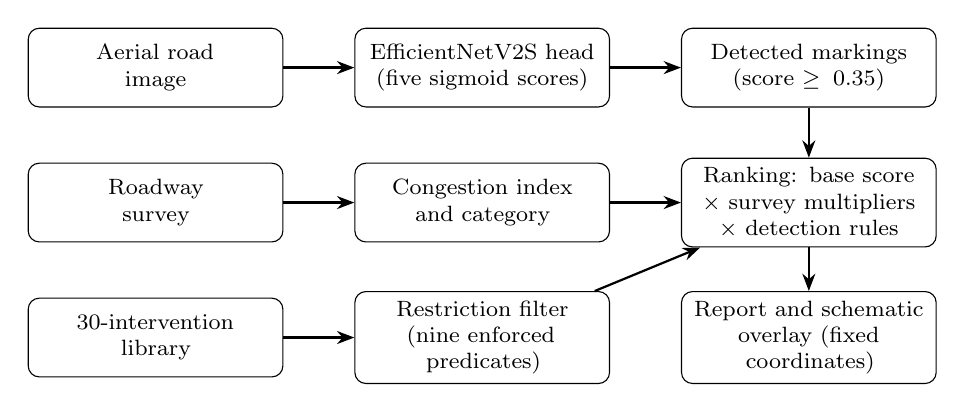
\begin{tikzpicture}[
  node distance=7mm and 9mm,
  box/.style={draw, rounded corners, align=center, font=\footnotesize, minimum height=10mm, text width=3.0cm},
  arr/.style={-{Stealth[length=2.2mm]}, thick}]
\node[box] (img) {Aerial road\\image};
\node[box, right=of img] (clf) {EfficientNetV2S head\\(five sigmoid scores)};
\node[box, right=of clf] (det) {Detected markings\\(score $\ge 0.35$)};
\node[box, below=of img] (srv) {Roadway\\survey};
\node[box, right=of srv] (cong) {Congestion index\\and category};
\node[box, right=of cong] (rank) {Ranking: base score\\$\times$ survey multipliers\\$\times$ detection rules};
\node[box, below=of srv] (lib) {30-intervention\\library};
\node[box, right=of lib] (flt) {Restriction filter\\(nine enforced\\predicates)};
\node[box, right=of flt] (rep) {Report and schematic\\overlay (fixed\\coordinates)};
\draw[arr] (img) -- (clf);
\draw[arr] (clf) -- (det);
\draw[arr] (det) -- (rank);
\draw[arr] (srv) -- (cong);
\draw[arr] (cong) -- (rank);
\draw[arr] (lib) -- (flt);
\draw[arr] (flt) -- (rank);
\draw[arr] (rank) -- (rep);
\end{tikzpicture}
\caption{Data flow of the revised system. Detected markings now enter the ranking as soft multipliers (Table~\ref{tab:rules}). In the archived version the analysis function accepted the detected-elements argument but never used it, so image labels and rule-derived recommendations met only in the report.}
\label{fig:dataflow}
\end{figure}

\subsection{Evaluation procedures for the archived artifacts}
\label{sec:archive-eval}
\paragraph{Log extraction.} I parsed every complete 20-epoch trace in the 2025 archive. There were thirteen, one of them an exact duplicate of the 12 April 00:45 run, which leaves twelve distinct runs. For each I report final-epoch training and validation AUC and loss, and per-epoch curves for two representative runs. The descriptive best epoch is the one with maximum validation AUC; minimum validation loss is reported separately. Because picking the run with the highest validation AUC uses the validation set, that number is not an unbiased estimate. I computed no confidence intervals for these logs, since per-image predictions and repeated runs under a frozen protocol do not exist.

\paragraph{Deterministic scenario and restriction audit.} I extracted the archived decision functions, intervention library, and filtering predicates unchanged from the source and executed them without TensorFlow or image processing. Four scenarios varied occupancy, speed, congestion-period reporting, and special events while holding the other survey inputs fixed at three lanes, a crosswalk, a bicycle lane, and capacity 30. The filtering function had nine explicit predicates. One (no HOV lanes) never fired because of a case mismatch, leaving eight effective predicates. I applied each of the nine separately and compared the surviving candidates with the unrestricted set of 30, then ran the same nine checks against the revised predicates.

\paragraph{Sensitivity analysis.} To test how robust the constraint-aware ranking is to visual noise, I ran a Monte Carlo simulation of 500 trials. The scenario was the Milton Avenue survey (two lanes, 17 of 30 vehicles, 56 km/h, peak period reported) with an active \texttt{no new lanes} restriction. In each trial I injected random false-positive detections (50\% probability per class, confidence uniform between 0.35 and 0.90) and recorded the top-ranked recommendation.

\paragraph{Qualitative output review.} I reviewed six exported images for overlay type, visible class labels, and displayed scores, transcribing score text by magnifying each screenshot. With no independent ground truth, I assigned no correctness, precision, or recall. I did not use the overlays to infer delay, capacity, crash risk, or constructability.

\section{Results}
\subsection{Archived training runs (2025)}
Table~\ref{tab:training-runs} lists all twelve distinct logs. Nine runs used the 16-class scheme, six without augmentation and three with it. Three later runs used the 20-class scheme with augmentation. For the 16-class scheme, final-epoch validation AUC ranged from 0.8548 to 0.8697; the six non-augmented runs averaged 0.8635 and the three augmented runs 0.8568. For the 20-class scheme, final-epoch validation AUC ranged from 0.9478 to 0.9605 (mean 0.9544), and validation loss from 0.1718 to 0.1860. The corresponding 16-class validation losses ranged from 0.4187 to 0.4367.

\begin{table}[p]
\centering\small
\caption{Final-epoch metrics for all twelve distinct archived 20-epoch training runs.}
\label{tab:training-runs}
\resizebox{\textwidth}{!}{%
\begin{tabular}{lccccccc}
\toprule
Run (2025) & Classes & Aug. & Train AUC & Val. AUC & Train loss & Val. loss & Val. acc. \\
\midrule
16 Mar 12:43 (a) & 16 & No & 0.8909 & 0.8665 & 0.4022 & 0.4280 & n/a \\
16 Mar 12:43 (b) & 16 & No & 0.9180 & 0.8675 & 0.3545 & 0.4187 & n/a \\
16 Mar 13:09 & 16 & No & 0.8830 & 0.8697 & 0.4060 & 0.4269 & n/a \\
16 Mar 13:22 & 16 & No & 0.9003 & 0.8590 & 0.3802 & 0.4300 & n/a \\
4 Apr 15:33 & 16 & No & 0.8972 & 0.8553 & 0.3795 & 0.4237 & n/a \\
4 Apr 16:38 & 16 & No & 0.8860 & 0.8631 & 0.4045 & 0.4238 & n/a \\
11 Apr 20:02 & 16 & Yes & 0.8439 & 0.8548 & 0.4614 & 0.4311 & 0.0625 \\
12 Apr 00:15 & 16 & Yes & 0.8360 & 0.8566 & 0.4683 & 0.4367 & 0.0625 \\
12 Apr 00:45 & 16 & Yes & 0.8273 & 0.8589 & 0.4693 & 0.4304 & 0.0625 \\
20 Apr 20:58 & 20 & Yes & 0.9313 & 0.9605 & 0.2290 & 0.1718 & 0.1875 \\
21 Apr 20:57 & 20 & Yes & 0.9288 & 0.9548 & 0.2391 & 0.1787 & 0.1875 \\
22 Apr 18:27 & 20 & Yes & 0.9129 & 0.9478 & 0.2594 & 0.1860 & 0.1875 \\
\midrule
16-class, no augmentation (mean of 6) & n/a & n/a & 0.8959 & 0.8635 & 0.3878 & 0.4252 & n/a \\
16-class, augmentation (mean of 3) & n/a & n/a & 0.8357 & 0.8568 & 0.4663 & 0.4327 & 0.0625 \\
20-class, augmentation (mean of 3) & n/a & n/a & 0.9243 & 0.9544 & 0.2425 & 0.1788 & 0.1875 \\
\bottomrule
\end{tabular}}
\vspace{2mm}
\begin{minipage}{0.98\textwidth}\footnotesize AUC = area under the ROC curve (Keras micro-average); loss = binary cross-entropy; Val. acc. = Keras accuracy metric on 16 validation images (not logged before 11 April). All runs used the three-block CNN, Adam at $10^{-4}$, batch size 16, and a sequential 80/20 split. These values describe CNN versions, not EfficientNetV2S. A thirteenth trace, an exact duplicate of the 12 April 00:45 run, is omitted.\end{minipage}
\end{table}

The 4 April run reached its maximum validation AUC (0.8611) and minimum validation loss (0.4230) at epoch 19, then finished at 0.8553 and 0.4237. Training AUC rose from 0.6411 to 0.8972, and the gap between training and validation went from a validation advantage of 0.1834 at epoch 1 to a training advantage of 0.0419 at epoch 20. The 20 April run peaked at a validation AUC of 0.9618 at epoch 12 and finished at 0.9605, with validation loss 0.1718 and training AUC 0.9313. In both runs the validation curve flattened early, and in the 20-class run the first-epoch validation AUC was already high (Figures~\ref{fig:curves} and~\ref{fig:auc-summary}). With 16 validation images, these results cannot separate overfitting from split composition or small-sample noise.

\begin{figure}[htbp]
\centering
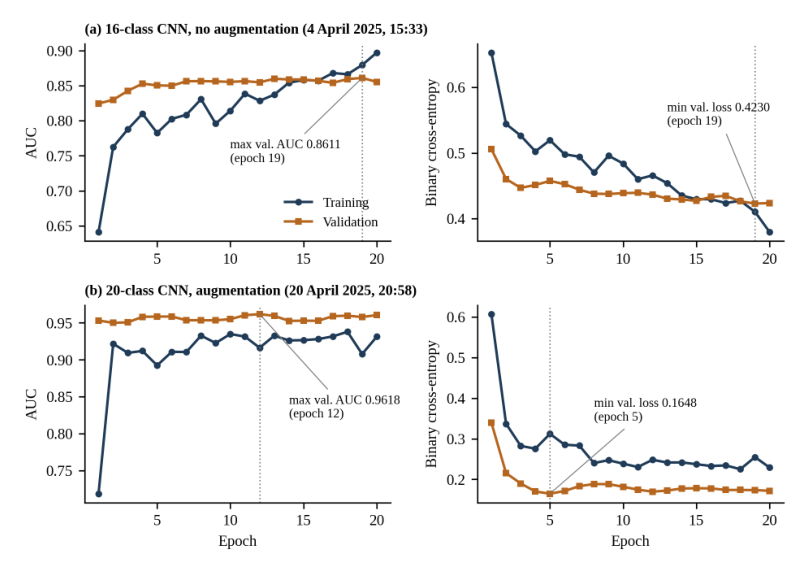
\includegraphics[width=0.82\textwidth]{figures/figure2_training_curves.png}
\caption{Training and validation curves for two representative archived runs. Panel (a) is the 4 April 16-class run: validation AUC peaks at epoch 19 while training AUC keeps rising. Panel (b) is the 20 April 20-class run: validation AUC is 0.953 at epoch 1 and stays in a narrow band; minimum validation loss (0.1648) occurs at epoch 5, and the final value is 0.1718. Dotted lines mark peak epochs. No independent test set or repeated frozen-protocol runs were available.}
\label{fig:curves}
\end{figure}

\begin{figure}[htbp]
\centering
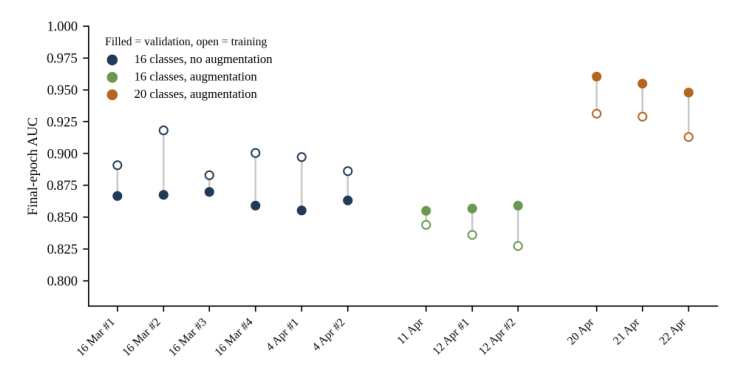
\includegraphics[width=0.72\textwidth]{figures/figure3_auc_summary.png}
\caption{Final-epoch training and validation AUC across all twelve archived runs. Each marker pair is one run, ordered by date within groups. The jump from the 16-class to the 20-class group coincides with a label-scheme change, and augmentation alone did not raise validation AUC. Other code changes mean the comparison does not isolate a single factor.}
\label{fig:auc-summary}
\end{figure}

\subsection{Interpreting the archived metrics}
\label{sec:metric-interpretation}
Three things limit what the 20-class result can show. First, the validation partition held 16 images, so accuracy values come in steps of $1/16$. The 20-class runs report 0.1875 (3/16) at the final epoch, the augmented 16-class runs report 0.0625 (1/16), and one epoch of the 20 April run reports 0.0. Those values fit a sample-level, exact-match-style measure and not ordinary per-label accuracy, but I could not verify the metric definition. Either way, exact label sets were rarely reproduced.

Second, the logged AUC is a micro-average over image--label pairs. Going to 20 classes adds many labels that are rare or absent in 76 images, and the extra easy negative pairs can raise pooled AUC and mean binary cross-entropy without improving recognition of the markings that do occur. The first-epoch validation AUC went from 0.8245 in the 16-class run to 0.9532 in the 20-class run, which fits that explanation, but the archive cannot confirm it because per-class metrics were never logged. Third, horizontal flipping in the augmentation turns a left-turn arrow into a right-turn arrow while leaving its label unchanged (corrected as R2).

The logs show a small network ranking labels above chance on a small validation split. They do not show dependable exact multi-label prediction, and the gain between label schemes cannot be credited to the model. I excluded a separate 20-value series labeled \texttt{avg\_accuracy} because its metric definition, dataset identity, and run linkage were missing.

\subsection{Cross-validated recognition performance of the revised pipeline}
\label{sec:cv-results}
\paragraph{Why a single split is not enough.} Before designing the cross-validation, I looked at two terminal traces of the earlier single-split EfficientNetV2S pipeline (61 training and 15 validation images, validation-based early stopping, identical code and data). They ended with validation AUC of 0.46 and 0.59 and exact-match accuracy of 1/15 in both. A gap of 0.13 between two runs of one configuration shows that a single 15-image split cannot support a performance claim, and it is why I adopted the protocol in Section~\ref{sec:cv-protocol}.

\paragraph{Overall performance.} Table~\ref{tab:cv-overall} gives all models on identical folds. The main model (head-only, label-swap flip) reached a macro AUC of 0.684 (95\% CI 0.63--0.73), with similar values across the three repeats (0.691, 0.667, 0.693). Macro AUC for single folds ranged from 0.553 to 0.798 (mean 0.705, SD 0.062 over 15 folds), which shows how much 15-image evaluation sets vary. The pooled out-of-fold value is lower than the mean fold value because pooling also penalizes score differences between folds. The prevalence baseline sits at 0.5 by construction, and HOG with logistic regression reached 0.646 (0.57--0.71). The linear probe on the same frozen features reached 0.738 (0.67--0.79), higher than every trained-head configuration. The main model's exact-match accuracy (0.184) equals the prevalence baseline's, and its BCE (0.620) is lower than the baseline's (0.666).

\begin{table}[htbp]
\centering\small
\caption{Out-of-fold performance on 76 images (5-fold iterative-stratified cross-validation $\times$ 3 repeats). Macro AUC with 95\% bootstrap CI; AP = average precision; exact match and BCE at the 0.35 threshold.}
\label{tab:cv-overall}
\resizebox{\textwidth}{!}{%
\begin{tabular}{lcccccc}
\toprule
Model & Macro AUC [95\% CI] & Fold AUC (mean $\pm$ SD) & AUC per repeat & Macro AP & Exact match & BCE \\
\midrule
\textbf{Main: head-only, label-swap flip} & 0.684 [0.63, 0.73] & 0.705 $\pm$ 0.062 & 0.691, 0.667, 0.693 & 0.739 & 0.184 & 0.620 \\
Naive flip (labels not swapped) & 0.663 [0.60, 0.72] & 0.690 $\pm$ 0.068 & 0.688, 0.694, 0.607 & 0.721 & 0.167 & 0.628 \\
No horizontal flip & 0.682 [0.62, 0.73] & 0.709 $\pm$ 0.056 & 0.694, 0.676, 0.676 & 0.745 & 0.175 & 0.621 \\
Fine-tune top 10 layers & 0.692 [0.63, 0.75] & 0.709 $\pm$ 0.053 & 0.700, 0.685, 0.693 & 0.736 & 0.180 & 0.612 \\
Fine-tune top 50 layers & 0.679 [0.62, 0.73] & 0.693 $\pm$ 0.063 & 0.690, 0.676, 0.670 & 0.740 & 0.189 & 0.616 \\
\midrule
Baseline: class prevalence & 0.500 [0.50, 0.50] & n/a & 0.500, 0.500, 0.500 & 0.579 & 0.184 & 0.666 \\
Baseline: HOG + logistic regression & 0.646 [0.57, 0.71] & 0.645 $\pm$ 0.062 & 0.662, 0.650, 0.624 & 0.679 & 0.127 & 0.912 \\
Baseline: linear probe (frozen features) & 0.738 [0.67, 0.79] & 0.734 $\pm$ 0.058 & 0.753, 0.741, 0.718 & 0.780 & 0.197 & 0.724 \\
\bottomrule
\end{tabular}}
\end{table}

\paragraph{Per-class performance.} Table~\ref{tab:cv-perclass} and Figure~\ref{fig:cv-auc} give per-class AUC with intervals. For the main model, the intervals for Left Turn Arrow, Right Turn Arrow, Stop Line, and Solid White Line lie entirely above 0.5, whereas the interval for Double Solid Yellow Line (0.575, 0.46--0.70) includes chance. That class is also the most prevalent (0.72), and its average precision of 0.769 is only slightly above the chance level of 0.724 (Table~\ref{tab:cv-ap}), which is weaker evidence than the AUC interval. The two baselines rank the classes differently: HOG scored highest on Double Solid Yellow Line (0.711), and the linear probe on Left Turn Arrow (0.787) and Solid White Line (0.820). With intervals this wide, per-class rankings among models are not reliable.

\begin{table}[htbp]
\centering\small
\caption{Per-class out-of-fold ROC AUC [95\% bootstrap CI]. Per-class results for the CNN ablations are in Appendix~E.}
\label{tab:cv-perclass}
\resizebox{\textwidth}{!}{%
\begin{tabular}{lccccc}
\toprule
Model & Left Turn Arrow & Right Turn Arrow & Stop Line & Solid White Line & Double Solid Yellow \\
\midrule
Main (head-only, label-swap flip) & 0.666 [0.56, 0.76] & 0.732 [0.65, 0.82] & 0.672 [0.56, 0.77] & 0.774 [0.68, 0.86] & 0.575 [0.46, 0.70] \\
HOG + logistic regression & 0.573 [0.45, 0.69] & 0.584 [0.46, 0.71] & 0.658 [0.54, 0.77] & 0.702 [0.59, 0.80] & 0.711 [0.56, 0.84] \\
Linear probe (frozen features) & 0.787 [0.68, 0.87] & 0.678 [0.56, 0.79] & 0.739 [0.62, 0.84] & 0.820 [0.72, 0.91] & 0.664 [0.52, 0.80] \\
\bottomrule
\end{tabular}}
\end{table}

\begin{table}[htbp]
\centering\small
\caption{Per-class average precision. The first row is the chance level (class prevalence).}
\label{tab:cv-ap}
\resizebox{\textwidth}{!}{%
\begin{tabular}{lccccc}
\toprule
Model & Left Turn Arrow & Right Turn Arrow & Stop Line & Solid White Line & Double Solid Yellow \\
\midrule
\emph{Chance (prevalence)} & 0.500 & 0.474 & 0.618 & 0.579 & 0.724 \\
Main (head-only, label-swap flip) & 0.662 & 0.702 & 0.753 & 0.808 & 0.769 \\
HOG + logistic regression & 0.537 & 0.525 & 0.744 & 0.760 & 0.831 \\
Linear probe (frozen features) & 0.773 & 0.644 & 0.815 & 0.840 & 0.830 \\
\bottomrule
\end{tabular}}
\end{table}

\begin{figure}[htbp]
\centering
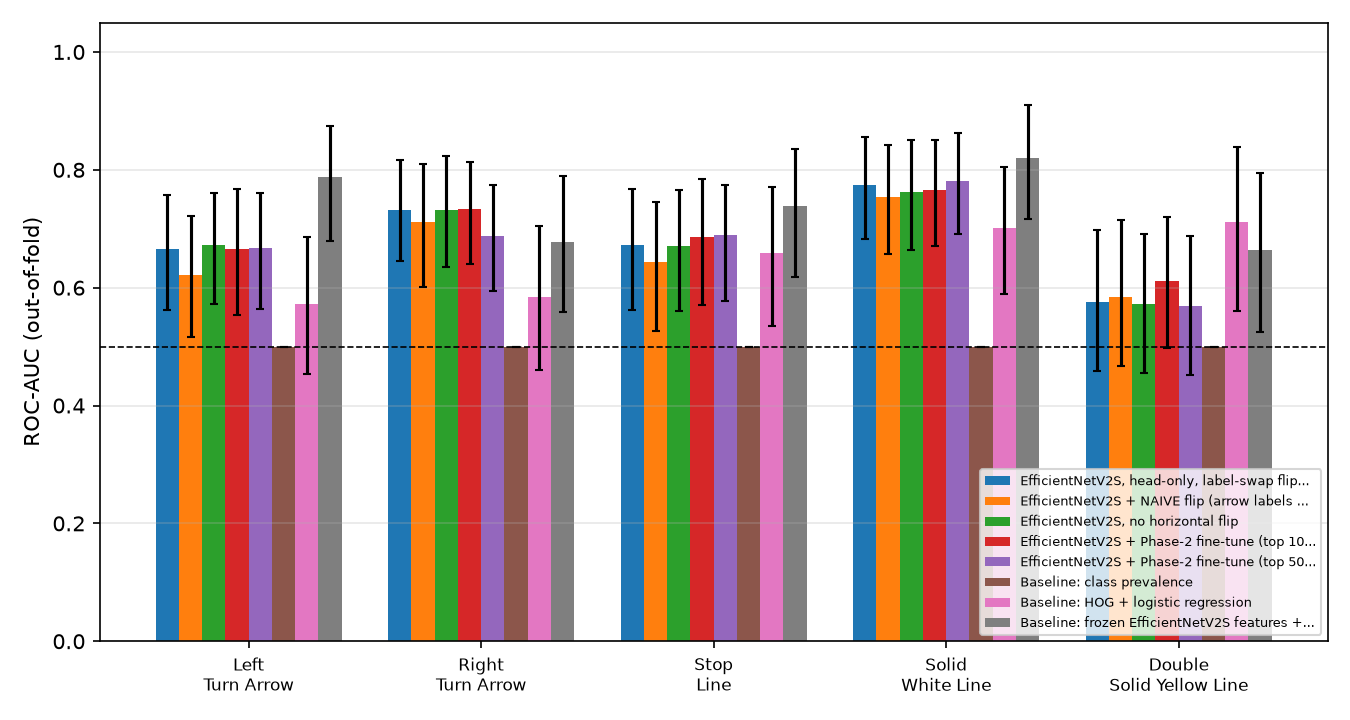
\includegraphics[width=0.95\textwidth]{figures/figure6_cv_auc.png}
\caption{Per-class out-of-fold ROC AUC with 95\% bootstrap intervals for the main model, four CNN variants, and three baselines (dashed line: chance). Intervals are wide and most models overlap within each class.}
\label{fig:cv-auc}
\end{figure}

\paragraph{Threshold-based outputs.} Table~\ref{tab:cv-thr} gives precision, recall, and F1 at the fixed 0.35 threshold. For the main model, recall is 0.98--1.00 for every class and precision is within about 0.05 of the class prevalence, so its positive predictions are no richer in true positives than the base rate. The model declares nearly every class present in nearly every image. Its exact-match accuracy and micro-F1 reproduce those of the prevalence baseline, and the left/right arrow swap rate of 0.030 means nothing because both arrows are predicted almost every time. The linear probe, whose scores are more spread out, reaches real precision and recall trade-offs. I therefore do not offer the CNN's thresholded outputs as evidence of recognition ability. The same threshold decides which detections trigger the ranking rules (Section~\ref{sec:integration}).

\begin{table}[htbp]
\centering\small
\caption{Precision / recall / F1 at threshold 0.35 (pooled out-of-fold predictions, mean over repeats).}
\label{tab:cv-thr}
\resizebox{\textwidth}{!}{%
\begin{tabular}{lccccc}
\toprule
Model & Left Turn Arrow & Right Turn Arrow & Stop Line & Solid White Line & Double Solid Yellow \\
\midrule
Main & 0.52 / 0.98 / 0.68 & 0.52 / 0.99 / 0.68 & 0.62 / 1.00 / 0.76 & 0.60 / 1.00 / 0.75 & 0.72 / 1.00 / 0.84 \\
Class prevalence & 0.50 / 1.00 / 0.67 & 0.47 / 1.00 / 0.64 & 0.62 / 1.00 / 0.76 & 0.58 / 1.00 / 0.73 & 0.72 / 1.00 / 0.84 \\
Linear probe & 0.65 / 0.83 / 0.73 & 0.58 / 0.68 / 0.63 & 0.71 / 0.85 / 0.77 & 0.74 / 0.92 / 0.82 & 0.76 / 0.90 / 0.82 \\
\bottomrule
\end{tabular}}
\end{table}

\paragraph{Paired comparisons and ablations.} Table~\ref{tab:cv-paired} reports paired differences (main minus alternative). The main model clearly beats the prevalence baseline (macro AUC difference 0.185, CI 0.13--0.23). Against HOG with logistic regression the macro difference is 0.039 (CI $-0.03$ to 0.10), so the two cannot be separated on macro AUC, though on the two arrow classes the main model is better by 0.122 (0.02--0.23). Against the linear probe the main model is worse by 0.053 (CI $-0.09$ to $-0.01$). All four ablations produced differences whose intervals contain zero. The naive flip scored 0.021 lower in macro AUC than the label-aware flip (CI $-0.01$ to 0.06; arrow classes 0.033, CI $-0.01$ to 0.08), which points toward label noise but cannot be told apart from zero here. Dropping the flip altogether changed nothing (0.002), and neither did unfreezing 10 or 50 backbone layers ($-0.008$ and 0.006). At this sample size the data support neither the necessity of the label correction nor any benefit from flipping or fine-tuning. The seven comparisons are not corrected for multiple testing, and the linear-probe result in particular would weaken under a conservative correction.

\begin{table}[htbp]
\centering\small
\caption{Paired differences, main model minus alternative (bootstrap, same resamples). Positive values favor the main model. $P_{\le}$ is the fraction of resamples in which the alternative matched or exceeded the main model; values are not multiplicity-corrected. Differences are computed from unrounded metrics and may differ in the last digit from differences of the rounded values in Table~\ref{tab:cv-overall}.}
\label{tab:cv-paired}
\begin{tabular}{lccc}
\toprule
Alternative & $\Delta$ macro AUC [95\% CI] & $\Delta$ arrow-class AUC [95\% CI] & $P_{\le}$ \\
\midrule
Naive flip & 0.021 [$-0.01$, 0.06] & 0.033 [$-0.01$, 0.08] & 0.093 \\
No horizontal flip & 0.002 [$-0.01$, 0.01] & $-0.003$ [$-0.03$, 0.02] & 0.373 \\
Fine-tune top 10 layers & $-0.008$ [$-0.03$, 0.01] & 0.001 [$-0.03$, 0.03] & 0.788 \\
Fine-tune top 50 layers & 0.006 [$-0.02$, 0.03] & 0.022 [$-0.01$, 0.05] & 0.312 \\
\midrule
Class prevalence & 0.185 [0.13, 0.23] & 0.199 [0.12, 0.26] & 0.000 \\
HOG + logistic regression & 0.039 [$-0.03$, 0.10] & 0.122 [0.02, 0.23] & 0.125 \\
Linear probe & $-0.053$ [$-0.09$, $-0.01$] & $-0.033$ [$-0.08$, 0.01] & 0.995 \\
\bottomrule
\end{tabular}
\end{table}

\subsection{Congestion scenarios (archived version)}
\label{sec:congestion-scenarios}
Table~\ref{tab:scenarios} gives four deterministic scenarios on the raw index scale of Equation~\ref{eq:congestion}. The code reproduced the arithmetic of the equation. In Scenario A, occupancy contributed 0.2833 and the speed term was zero because 56 km/h exceeds 50 km/h. Adding a reported peak period raised the index to 0.3833, still under the 0.4 threshold. Scenario C crossed into Congested, and two special events moved Scenario D to Severely Congested. Signal-related options rose in rank when a peak period activated their multiplier. Scenarios A and B still returned three candidates, so the implementation behaves as a general option generator and not as a recommender gated on congestion. The revised normalization (R5) leaves these categories unchanged.

\begin{table}[htbp]
\centering\small
\caption{Deterministic outcomes of four survey scenarios (archived ranking, no detection rules).}
\label{tab:scenarios}
\begin{tabularx}{\textwidth}{P{0.25\textwidth} P{0.09\textwidth} P{0.15\textwidth} Y}
\toprule
Scenario & Index $C$ & Category & Top-ranked candidates, in order \\
\midrule
A. 17/30 vehicles; 56 km/h; no period or events & 0.2833 & Not Congested & Add roundabout; coordinate signal systems; convert to bike lane \\
B. As A, with a reported peak period & 0.3833 & Not Congested & Coordinate signal systems; add adaptive signals; add pedestrian signals \\
C. 24/30 vehicles; 40 km/h; peak period & 0.5600 & Congested & Coordinate signal systems; add adaptive signals; optimize signal timing; add pedestrian signals \\
D. As C, plus two special events & 0.7600 & Severely Congested & Coordinate signal systems; add adaptive signals; optimize signal timing; add roundabout; add pedestrian signals \\
\bottomrule
\end{tabularx}
\begin{minipage}{0.98\textwidth}\footnotesize All scenarios used capacity 30, three lanes, a crosswalk, and a bicycle lane. Rankings follow the coded weights and multipliers, including the 1.1 signal multiplier when a peak period is reported. Candidates are heuristic outputs, not recommended engineering actions.\end{minipage}
\end{table}

\subsection{Restriction-implementation audit}
\label{sec:restriction-audit}
The library lists 48 restriction strings (Appendix~C), but the archived filtering function had explicit predicates for only nine. The other 39 selectable restrictions did nothing. Table~\ref{tab:restrictions} shows the result of applying each implemented restriction separately in the archived and revised versions. In the archived version, eight predicates changed the candidate set.

The archived no HOV lanes predicate removed nothing. It searched for uppercase HOV inside an intervention name that had already been lowercased, so the match could never succeed and Convert to HOV lane stayed eligible; the revised predicate removes it. The no new lanes predicate removes five options, including Add bike lane markings, because it matches any name containing both \emph{lane} and \emph{add}. That lexical rule reaches beyond the three lane-addition records and dedicated turn lanes it was presumably meant to cover, and I left it unchanged. All nine checks of the revised predicates matched their expected removal counts when run on my machine. The revised interface offers only these nine restrictions. The other 39 remain in the catalogue but cannot be selected, so the interface no longer promises constraints it cannot enforce.

\begin{table}[htbp]
\centering\small
\caption{Single-restriction ablation against the unrestricted 30-option library, archived and revised predicates.}
\label{tab:restrictions}
\begin{tabularx}{\textwidth}{P{0.20\textwidth} P{0.11\textwidth} P{0.11\textwidth} Y}
\toprule
Applied restriction & Remaining (archived) & Remaining (revised) & Candidates removed (revised) \\
\midrule
No new lanes & 25 & 25 & Add general-purpose lane; add auxiliary lane; add climbing lane; add dedicated turn lanes; add bike lane markings \\
No construction & 19 & 19 & Eleven physical options with cost $>0.4$ \\
No overpasses & 28 & 28 & Pedestrian overpass; vehicle overpass \\
No underpasses & 29 & 29 & Pedestrian underpass \\
No bike lanes & 28 & 28 & Convert to bike lane; add bike lane markings \\
No bus lanes & 29 & 29 & Convert to bus lane \\
No HOV lanes & 30 & \textbf{29} & Convert to HOV lane (archived: none; case-sensitive predicate never matched) \\
No signal timing changes & 29 & 29 & Optimize signal timing \\
No pedestrian signals & 29 & 29 & Add pedestrian signals \\
\bottomrule
\end{tabularx}
\begin{minipage}{0.98\textwidth}\footnotesize Each restriction was tested independently. Of the 48 labels, nine have explicit predicates; the remaining 39 have no enforcement logic and are not verified constraints. HOV = high-occupancy vehicle.\end{minipage}
\end{table}

\subsection{Integration of detected markings}
\label{sec:integration}
In the archived version, the \texttt{analyze\_traffic} function accepted a \texttt{detected\_elements} argument and never referenced it, so changing image labels left $C$, the candidate set, and the ranking untouched. That was an integration gap in the artifact, not an estimate of model error. The revised function applies the rules in Table~\ref{tab:rules}.

Table~\ref{tab:integration} shows the effect for the Milton Avenue survey (two lanes, 17 of 30 vehicles, 56 km/h, peak period 8--9 AM, crosswalk and bicycle lane present, no restrictions; index 0.3833 raw, displayed as 0.32). In the revised system's run on a test image, all three rules fired because Left Turn Arrow, Right Turn Arrow, Stop Line, and Double Solid Yellow Line all scored above 0.35. I reproduced the rankings by evaluating the coded scoring rules (Tier~3), and the three options the system reports for this survey match its printed output. Detection moved Add dedicated turn lanes from third place to first. The turn-arrow rule also multiplies Add turn arrows, but that option (computed score 0.715) stays outside the top five. Because the CNN's scores exceed the 0.35 threshold for almost every class in almost every image (Table~\ref{tab:cv-thr}), the rules fire nearly regardless of image content, and the ranking's dependence on the image is weak at present.

To see how visual noise affects the final output, I ran the Monte Carlo sensitivity analysis described in Section~\ref{sec:archive-eval} (500 trials, random false-positive detections). The top recommendation, \emph{Convert to bike lane}, did not change in any trial. The reason is constraint ordering. The \texttt{no new lanes} restriction removed \emph{Add dedicated turn lanes}, the candidate most boosted by arrow detections, before ranking. False positives could still raise other candidates, but none passed the top-ranked option. In this case the constraint kept noisy visual input from changing the primary recommendation. The result depends on that removal: in the unrestricted case of Table~\ref{tab:integration}, the same detections do change the top recommendation.

\begin{table}[htbp]
\centering\small
\caption{Top five candidates for the Milton Avenue survey, without and with the detection rules (computed score in parentheses). The system reports the top three for this congestion level.}
\label{tab:integration}
\begin{tabularx}{\textwidth}{c Y Y}
\toprule
Rank & Without detection rules & With rules for turn arrows, stop line, and double solid yellow line \\
\midrule
1 & Convert to bike lane (0.835) & Add dedicated turn lanes (0.886) \\
2 & Coordinate signal systems (0.814) & Convert to bike lane (0.835) \\
3 & Add dedicated turn lanes (0.805) & Coordinate signal systems (0.814) \\
4 & Add bike lane markings (0.797) & Add pedestrian signals (0.813) \\
5 & Add adaptive signals (0.792) & Optimize signal timing (0.809) \\
\bottomrule
\end{tabularx}
\end{table}

An early Milton Avenue session in the archived version also shows how the system's description of congestion can disagree with the user's. The user entered High, but 17 of 30 vehicles, 56 km/h, and no reported period or special events give $C=0.283$ and the category Not Congested. The calculation follows the coded rule. The interface did not reconcile the user's label with the computed category, and I did not change that.

\subsection{Qualitative visualization outputs}
The six images from the archived versions show bus-lane, roundabout, turn-lane, pedestrian-overpass, bicycle-lane, and signal-optimization graphics on several road scenes (Figures~\ref{fig:outputs-a} and~\ref{fig:outputs-b}). Five display four numerical marking scores. The sixth, dated 13 April 2025, predates the final label scheme and lists Car, Crosswalk, and Solid White Line without scores. Table~\ref{tab:display-scores} transcribes the visible scores. The archive does not say which model version produced each image, since it holds several class schemes and no model-version manifest. File timestamps are 13 April, 22 April (three images), and 4 July 2025, plus one undated image.

\begin{table}[htbp]
\centering\small
\caption{Model-reported scores visible in the six archived output images.}
\label{tab:display-scores}
\footnotesize
\begin{tabularx}{\textwidth}{P{0.18\textwidth} >{\centering\arraybackslash}p{0.11\textwidth} >{\centering\arraybackslash}p{0.11\textwidth} >{\centering\arraybackslash}p{0.11\textwidth} >{\centering\arraybackslash}p{0.11\textwidth} Y}
\toprule
Panel & Double solid yellow (\%) & Solid white (\%) & Left-turn arrow (\%) & Right-turn arrow (\%) & Displayed overlay \\
\midrule
(a) Bus-lane overlay & 86.5 & 63.9 & 66.2 & 46.6 & Bus-lane band \\
(b) Roundabout, intersection & 93.5 & 85.3 & 59.0 & 53.0 & Roundabout circle \\
(c) Roundabout, tree-covered scene & 83.3 & 75.3 & 67.1 & 41.2 & Roundabout circle \\
(d) Turn-lane overlay & 85.1 & 81.1 & 68.1 & 44.1 & Turn-lane box \\
(e) Milton Avenue & 69.8 & 71.8 & 61.7 & 43.1 & Turn-lane box; optimized marker \\
(f) Combined overlays & n/a & n/a & n/a & n/a & Overpass, bike lane, turn lane \\
\bottomrule
\end{tabularx}
\begin{minipage}{0.98\textwidth}\footnotesize Scores are transcribed from the interface; they are not accuracy metrics or calibrated probabilities. Panel (f) displays Car, Crosswalk, and Solid White Line without scores. Stop line does not appear because only four entries are displayed.\end{minipage}
\end{table}

Visible scores ranged from 41.2\% to 93.5\%, and the right-turn-arrow score exceeded the 0.35 inference threshold in every image. In the tree-covered Milton Avenue crops (panels a, c, and e) I could see no painted arrows, though canopy hid much of the pavement. This describes the display and is not an error rate. Without independent annotations, the predictions cannot be marked correct or incorrect. In the intersection scenes (panels b and d) two painted turn arrows are visible, and the model's left- and right-turn scores differ by 6 and 24 points respectively. I did not score these against the painted direction, and a single scene says nothing about detection accuracy. The overlays use fixed coordinates: the roundabout circle in panel (b) sits on an existing intersection with marked crosswalks, and the turn-lane box in panel (e) occupies a fixed image position unrelated to pavement geometry.

The revised system, using a model trained on all 76 images, listed all five classes above the threshold for a Milton Avenue test image, with scores of 82.6\% (Solid White Line), 75.9\% (Stop Line), 73.7\% (Double Solid Yellow Line), 58.7\% (Left Turn Arrow), and 47.3\% (Right Turn Arrow). That matches the cross-validated finding that the 0.35 threshold admits nearly every class. Because this model had seen all the labeled data, the scores say nothing about accuracy.

\begin{figure}[p]
\centering
\begin{subfigure}[t]{0.98\textwidth}\centering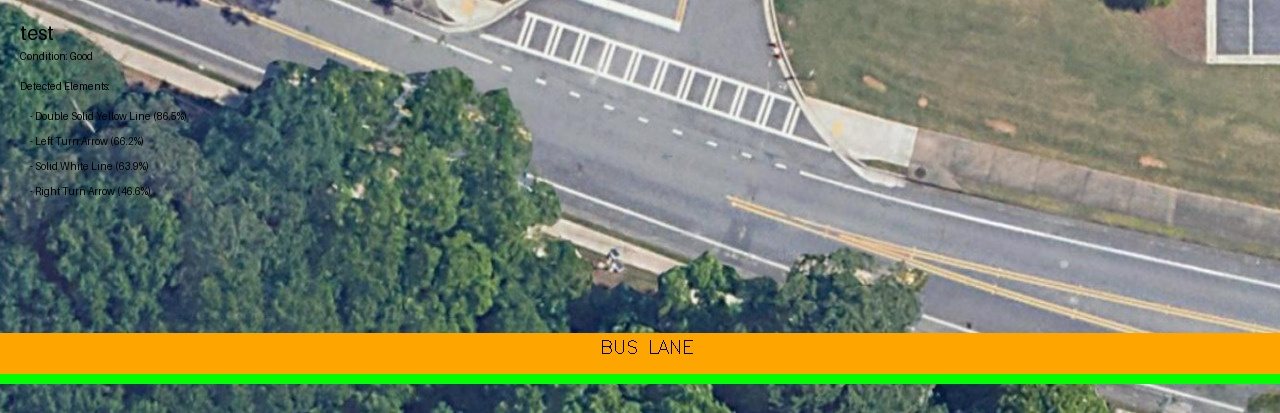
\includegraphics[width=\linewidth,height=0.22\textheight,keepaspectratio]{figures/figure4a_bus_lane.jpg}\caption{Bus-lane overlay}\end{subfigure}\par\smallskip
\begin{subfigure}[t]{0.98\textwidth}\centering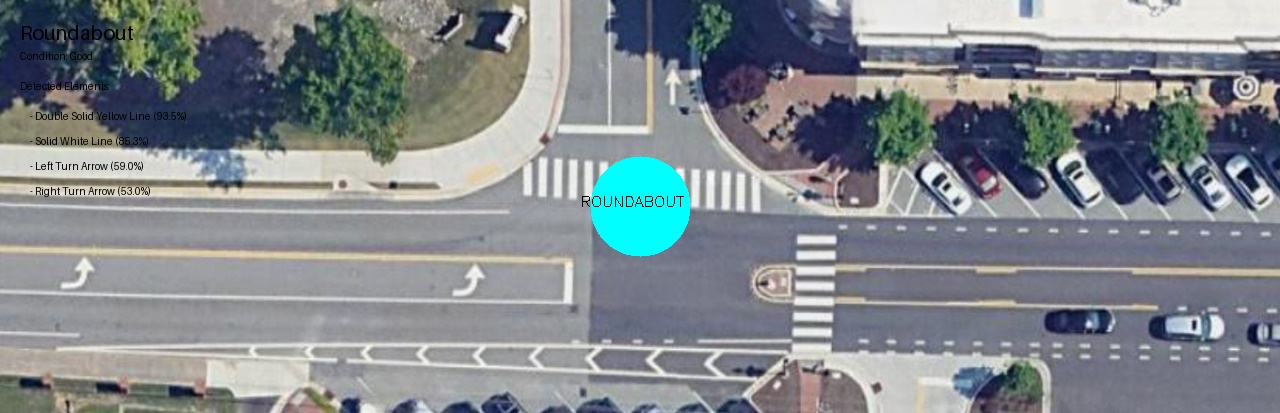
\includegraphics[width=\linewidth,height=0.22\textheight,keepaspectratio]{figures/figure4b_roundabout_intersection.jpg}\caption{Roundabout, intersection scene}\end{subfigure}\par\smallskip
\begin{subfigure}[t]{0.98\textwidth}\centering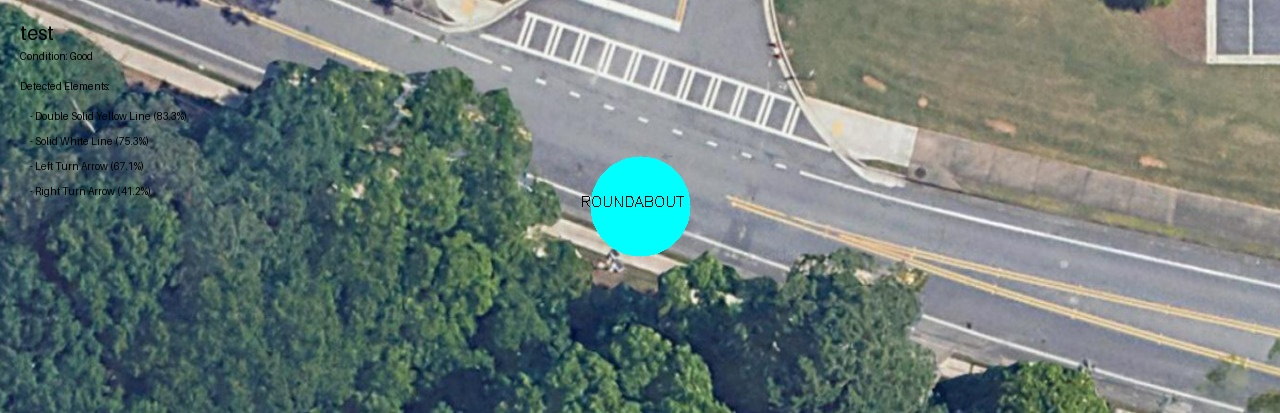
\includegraphics[width=\linewidth,height=0.22\textheight,keepaspectratio]{figures/figure4c_roundabout_trees.jpg}\caption{Roundabout, tree-covered scene}\end{subfigure}
\caption{Archived outputs illustrating schematic interventions, panels (a)--(c). Colored shapes and text are drawn by the application at fixed image-relative positions. These outputs have no independent ground truth and do not validate detection correctness, design geometry, or traffic effects. Imagery \copyright{} 2026 Vexcel Imaging US, Inc., Airbus, Maxar Technologies; map data \copyright{} 2026 Google.}
\label{fig:outputs-a}
\end{figure}

\begin{figure}[p]
\centering
\renewcommand{\thesubfigure}{\ifcase\value{subfigure}\or d\or e\or f\fi}
\begin{subfigure}[t]{0.98\textwidth}\centering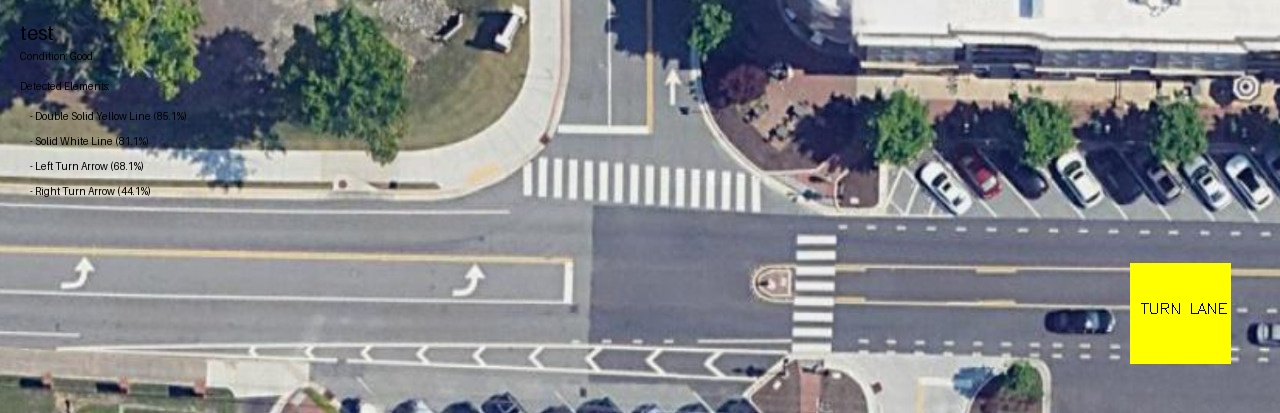
\includegraphics[width=\linewidth,height=0.22\textheight,keepaspectratio]{figures/figure5d_turn_lane.jpg}\caption{Turn-lane overlay, intersection scene}\end{subfigure}\par\smallskip
\begin{subfigure}[t]{0.98\textwidth}\centering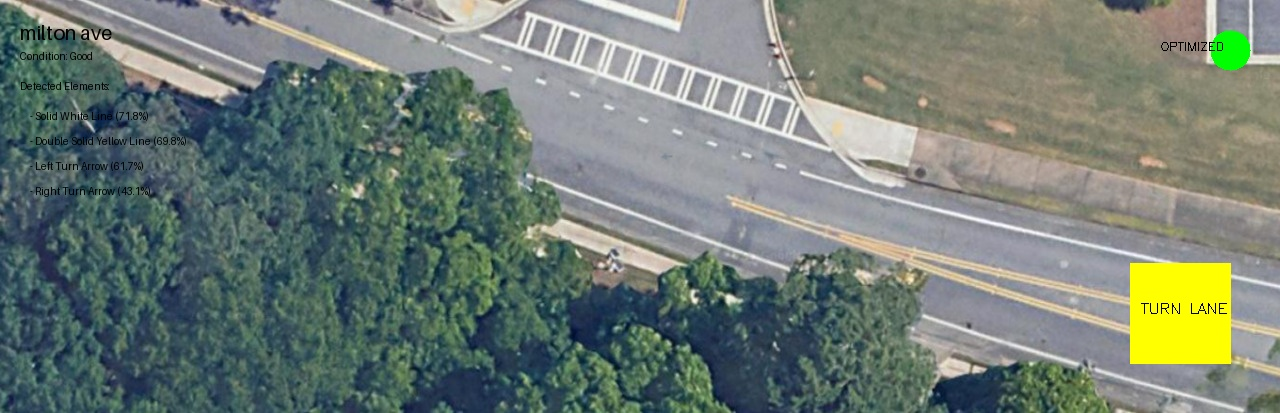
\includegraphics[width=\linewidth,height=0.22\textheight,keepaspectratio]{figures/figure5e_milton.jpg}\caption{Milton Avenue: turn-lane and optimized graphics}\end{subfigure}\par\smallskip
\begin{subfigure}[t]{0.98\textwidth}\centering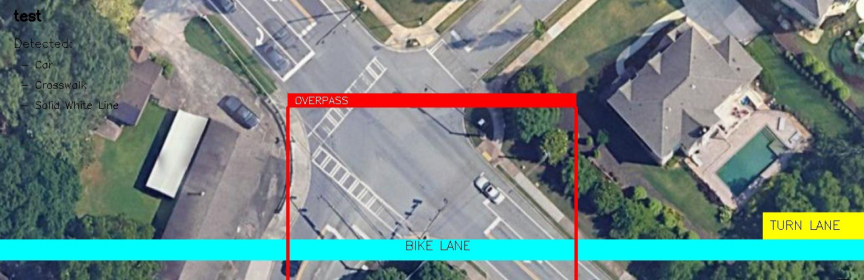
\includegraphics[width=\linewidth,height=0.22\textheight,keepaspectratio]{figures/figure5f_combined.png}\caption{Combined overpass, bicycle-lane, and turn-lane graphics}\end{subfigure}
\caption{Archived outputs illustrating schematic interventions, panels (d)--(f); notes as in Figure~\ref{fig:outputs-a}. Panel (f) came from an earlier interface version and lists Car, Crosswalk, and Solid White Line without scores. Imagery \copyright{} 2026 Vexcel Imaging US, Inc., Airbus, Maxar Technologies; map data \copyright{} 2026 Google.}
\label{fig:outputs-b}
\end{figure}

\section{Discussion}
\subsection{What the artifact does and does not show}
The reconstruction supports a narrow conclusion. Multi-label recognition, structured roadway attributes, heuristic congestion categories, intervention ranking, and visualization can be built as separate modules and combined in one report. Deterministic audits can expose gaps between intended and actual behavior before any field evaluation, and the fixes that follow can be verified the same way. A plausible overlay or ranked list is not evidence of transportation value. The prototype is a research artifact and a communication scaffold, and its decision logic is provisional.

The detected-elements gap resembles the glue-code and pipeline-integration problems \citet{sculley2015} describe for machine-learning systems, where components work alone while the connections between them go untested. Wiring the classifier into the ranking closed that gap and exposed the next one: the connection means something only if the classifier's outputs discriminate, and at the fixed threshold they do not.

\subsection{Recognition results}
With 76 images, a frozen ImageNet EfficientNetV2S backbone with a trained sigmoid head ranks images by the presence of four of the five marking classes better than chance (macro AUC 0.684). That is all the data support. They do not support a claim of accurate road-marking detection. Four points qualify the result.

First, the trained head did not beat a regularized logistic regression on the same frozen features, and the paired difference excludes zero. Possible reasons are the head's augmentation, its fixed schedule, and batch normalization on very small training folds, while the probe uses standardized features and strong L2 regularization. I tested none of these, and the comparison should not be extended to larger datasets. Because I found the probe's advantage after fixing the main configuration, choosing it as the recognition component would be a post hoc decision that needs confirmation on new data.

Second, the CNN's scores are unusable at the 0.35 threshold. A deployment threshold should be chosen in an inner cross-validation loop or on a separate calibration set, and ranking metrics (AUC, AP) are the right summaries here. Third, Double Solid Yellow Line could not be told apart from chance for the CNN, although a hand-crafted baseline did better on it. Thin, long marking structures may be poorly represented after resizing to 224 pixels. The code specifies a higher-resolution ablation that I did not run. Fourth, the earlier 20-class gain in micro-averaged AUC (Section~\ref{sec:metric-interpretation}) should not be compared with these per-class, five-class results.

I chose the main configuration (fixed 20 epochs, head-only training, prior-initialized output bias) after exploratory single-split runs on the same 76 images, in which fine-tuning seemed to lower validation AUC. I tuned no hyperparameter inside the cross-validation, but the configuration is not free of selection on this dataset. Cross-validation also cannot remove leakage between images of the same road that are not near-duplicates, and location-disjoint splits need location metadata the archive does not have.

\subsection{Decision rules}
The scenario checks show that rankings respond to hand-designed multipliers. A reported peak period adds 0.1 to the congestion index and multiplies every signal-related score by 1.1, and Add pedestrian signals can receive both the pedestrian and the signal multiplier. That is why signal options dominated the tested scenarios. It does not show that signal optimization is the most effective treatment. The detection rules in Table~\ref{tab:rules} are equally arbitrary in size, and in most cases they move rankings by only a few hundredths of a score point (Table~\ref{tab:integration}). The sensitivity analysis in Section~\ref{sec:integration} showed that, in the tested scenario, a hard constraint protected the top recommendation from spurious detections, because it removed the one candidate that false positives would have helped. Whether that holds across more scenarios, several interacting constraints, and less dominant top candidates is untested. Future work should also vary the weights and multipliers over plausible ranges and replace unvalidated point values with expert or stakeholder elicitation where possible.

Evidence on roundabouts and bicycle safety shows that outcomes depend on site and design characteristics \citep{gross2013,poudel2021}. A ranking system should encode applicability conditions and uncertainty instead of multiplying generic scores. Candidate generation can stay broad, but any operational recommendation would need assessment of demand, delay, safety, accessibility, environmental effects, cost, and right of way.

\subsection{Constraint handling as a verification problem}
The restriction audit shows that displaying a list of constraints is different from enforcing them. In the archived version only nine of 48 restrictions had predicates, and one of those was ineffective. The revision changes what the interface promises: it offers only enforced restrictions. That is more honest but smaller, and enforcing the other 39 would need structured intervention attributes instead of name matching. The broad no new lanes rule also removes bicycle-lane markings, a clear case of lexical matching excluding something it should not.

A maintainable implementation would describe interventions with structured attributes and each restriction with a formal, unit-tested rule. Tests should cover every restriction, synonyms, missing values, conflicting restrictions, and unintended removals, and the output should say why each candidate was excluded.

\section{Limitations}
\label{sec:limitations}
The main limitation is uneven provenance. The training images and annotations are in a public repository, and class frequencies can be recovered by parsing them, but the number of distinct locations is not recorded and no location metadata is attached to individual images. Model weights from the archived 2025 runs are lost, so those results cannot be reproduced exactly. The archived validation partition was sequential and held 16 images, and the twelve archived runs differ in label scheme, augmentation, and other code details, so cross-run comparisons are descriptive.

The cross-validated evaluation has its own limits. It uses 76 images with 15--16 per fold, intervals are wide, and per-class rankings among models are unreliable. The bootstrap treats images as independent apart from the near-duplicate grouping. The three repeats share the same images and are not independent samples, so seed variation is only partly captured. Seven paired comparisons were made without multiplicity correction. The main configuration was informed by exploratory runs on the same data. There is no independent external test set, no location-disjoint split, and no calibration analysis. Merging straight-or-left arrows into Left Turn Arrow (seven objects) is a labeling decision. The label-aware flip assumes that the mirror image of a left-turn arrow is a right-turn arrow, and it also produces mirrored scene geometry that never occurs under right-hand traffic. The HOG baseline is a NumPy re-implementation, not the OpenCV descriptor.

Several defects were identified and left unfixed. The speed term is skipped when speed is zero. The no new lanes rule over-matches and removes bicycle-lane markings. Inspection of the survey code (Tier~1) shows that the special-events prompt asks the user twice, once for the gate and once for the value, so contradictory answers can change $e$ in Equation~\ref{eq:congestion}. The user-entered congestion label is not reconciled with the computed category. Some code comments still refer to 20 classes, and the early 16-class scheme has near-duplicate labels. Outputs should record the model, class-schema, and dataset versions, and the system does not yet do so.

The decision model is heuristic. Capacity, speed thresholds, category cutoffs, impact, safety, cost, multipliers, and detection-rule factors were not estimated from observed traffic outcomes, and several collected attributes do not affect decisions. Fixed-coordinate overlays do not encode road geometry. The study includes no usability experiment, expert review, runtime benchmark, equity assessment, simulation, before--after crash analysis, or field congestion measurement. Figure imagery is attributed in the figure notes, and this paper does not redistribute the underlying dataset.

\section{Future Work}
The first priority is a versioned evaluation dataset with location-disjoint training, validation, and test partitions, an untouched test set, and location metadata recorded at capture time. The recognition module should then be compared again against a linear probe on frozen features, since that baseline was not beaten here; if it stays competitive, the simpler model is the better choice. Class-specific precision--recall analysis, calibration, a threshold chosen by nested cross-validation, and higher-resolution input (especially for line markings) should follow, along with error analysis across weather, illumination, camera angle, occlusion, and marking wear. Each prediction should be tied to a model hash, dataset version, threshold, and ground-truth status.

The decision layer should be rebuilt around explicit intervention attributes and a complete constraint registry. Image-derived features should either stay descriptive or enter recommendations through tested rules, and only after the corresponding classes have been validated. Weight and threshold sensitivity, expert agreement, and explanation quality need evaluation before any operational use. Geometry-aware visualizations should rest on segmentation or surveyed geometry and be checked against the applicable design standards.

The deterministic scenario checks in Section~\ref{sec:congestion-scenarios} give a limited, controlled comparison of rankings under varying survey inputs. They are single-point heuristic evaluations that do not model dynamic traffic and cannot replace calibrated microsimulation. Claims about transportation value would need outcome evaluation: simulation where feasible, then site-specific before--after studies of delay, speed reliability, throughput, safety, accessibility, and unintended effects, with measurement protocols that protect privacy. Human-in-the-loop studies should test whether users understand that scores and overlays are provisional. Only after that could the system support claims about recommendation quality or congestion mitigation.

\section{Conclusion}
The reconstructed prototype demonstrates a modular approach to multi-label road-marking reporting, survey-driven congestion categorization, intervention ranking, and schematic visualization. Twelve archived training logs show that a compact CNN trained on 76 map screenshots ranked labels above chance on a 16-image validation split, but the jump from the 16-class to the 20-class scheme cannot be credited to better recognition. A deterministic audit found incomplete restriction enforcement, an ineffective HOV filter, and an analysis function that ignored detected markings. I fixed these, along with a label-inconsistent flip augmentation, annotation spelling mismatches, and silent data fallbacks. Under repeated cross-validation, the revised EfficientNetV2S head reached a macro AUC of 0.684 (95\% CI 0.63--0.73), could not be distinguished from chance on Double Solid Yellow Line, lost to a logistic-regression probe on the same frozen features (0.738), and produced scores above the fixed 0.35 threshold for nearly every class.

The artifact is a feasible proof of concept and a starting point for verification research. It is not a validated traffic-management system. Claims about recognition performance, safe design, user value, or congestion reduction would need versioned data, independent location-disjoint testing, complete constraint verification, geometry-aware visualization, and evaluation against transportation outcomes.

\section*{Data and Code Availability}
\phantomsection
\label{sec:data-code}
I extracted the archived numerical results from terminal logs and from deterministic execution of the archived decision code. The training images, Pascal VOC annotations, source code, and exported output images are public at \url{https://github.com/KingFarooq/TrafficCongestionWithAI}. The same repository holds the revised pipeline, unit tests, fold assignments, configuration files, out-of-fold predictions, and result tables for the cross-validated experiments. The aerial base imagery is third-party material (Google, Vexcel Imaging US, Maxar Technologies) and is subject to those providers' terms of use; redistribution downstream is the reader's responsibility. This paper reproduces the per-run values behind Table~\ref{tab:training-runs}, the full intervention library (Appendix~B), the restriction catalogue (Appendix~C), and the annotation vocabulary (Appendix~D). No preregistered analysis plan exists for this study.

\section*{Declarations}
\noindent\textbf{Funding:} The author received no specific funding for this work.\par
\noindent\textbf{Competing interests:} The author declares none.\par
\noindent\textbf{Ethics:} No human participants or personal data were involved.

\begin{thebibliography}{99}
\bibitem[Alain and Bengio(2017)]{alain2017} Alain, G., \& Bengio, Y. (2017). Understanding intermediate layers using linear classifier probes. \emph{arXiv preprint arXiv:1610.01644}. \url{https://arxiv.org/abs/1610.01644}
\bibitem[Dalal and Triggs(2005)]{dalal2005} Dalal, N., \& Triggs, B. (2005). Histograms of oriented gradients for human detection. In \emph{Proceedings of the IEEE Conference on Computer Vision and Pattern Recognition} (Vol. 1, pp. 886--893). IEEE. \url{https://doi.org/10.1109/CVPR.2005.177}
\bibitem[Efron and Tibshirani(1993)]{efron1993} Efron, B., \& Tibshirani, R. J. (1993). \emph{An introduction to the bootstrap}. Chapman \& Hall.
\bibitem[Everingham et~al.(2010)]{everingham2010} Everingham, M., Van Gool, L., Williams, C. K. I., Winn, J., \& Zisserman, A. (2010). The PASCAL Visual Object Classes (VOC) Challenge. \emph{International Journal of Computer Vision, 88}(2), 303--338. \url{https://doi.org/10.1007/s11263-009-0275-4}
\bibitem[Federal Highway Administration(2015)]{fhwa2015} Federal Highway Administration. (2015). \emph{Engineering around the school: Safe Routes to School online guide}. U.S. Department of Transportation. \url{https://highways.dot.gov/safety/pedestrian-bicyclist/safety-tools/engineering-around-school-safe-routes-school-online-guide}
\bibitem[Gross et~al.(2013)]{gross2013} Gross, F., Lyon, C., Persaud, B., \& Srinivasan, R. (2013). Safety effectiveness of converting signalized intersections to roundabouts. \emph{Accident Analysis \& Prevention, 50}, 234--241. \url{https://doi.org/10.1016/j.aap.2012.04.012}
\bibitem[Guo et~al.(2017)]{guo2017} Guo, C., Pleiss, G., Sun, Y., \& Weinberger, K. Q. (2017). On calibration of modern neural networks. In \emph{Proceedings of the 34th International Conference on Machine Learning} (Vol. 70, pp. 1321--1330). PMLR. \url{https://proceedings.mlr.press/v70/guo17a.html}
\bibitem[He and Balakrishnan(2022)]{he2022} He, S., \& Balakrishnan, H. (2022). Lane-level street map extraction from aerial imagery. In \emph{Proceedings of the IEEE/CVF Winter Conference on Applications of Computer Vision} (pp. 2080--2089). IEEE.
\bibitem[Hevner et~al.(2004)]{hevner2004} Hevner, A. R., March, S. T., Park, J., \& Ram, S. (2004). Design science in information systems research. \emph{MIS Quarterly, 28}(1), 75--105. \url{https://doi.org/10.2307/25148625}
\bibitem[Institute of Transportation Engineers(2012)]{ite2012} Institute of Transportation Engineers. (2012). \emph{School area traffic control}. Safe Routes to School Online Resource Library.
\bibitem[Jayasinghe et~al.(2022)]{jayasinghe2022} Jayasinghe, O., Hemachandra, S., Anhettigama, D., Kariyawasam, S., Rodrigo, R., \& Jayasekara, P. (2022). CeyMo: See more on roads: A novel benchmark dataset for road marking detection. In \emph{Proceedings of the IEEE/CVF Winter Conference on Applications of Computer Vision} (pp. 3104--3113). IEEE.
\bibitem[Kingma and Ba(2015)]{kingma2015} Kingma, D. P., \& Ba, J. (2015). Adam: A method for stochastic optimization. In \emph{3rd International Conference on Learning Representations}. \url{https://arxiv.org/abs/1412.6980}
\bibitem[Lee et~al.(2017)]{lee2017} Lee, S., Kim, J., Shin Yoon, J., Shin, S., Bailo, O., Kim, N., Lee, T.-H., Seok Hong, H., Han, S.-H., \& So Kweon, I. (2017). VPGNet: Vanishing point guided network for lane and road marking detection and recognition. In \emph{Proceedings of the IEEE International Conference on Computer Vision} (pp. 1947--1955). IEEE.
\bibitem[Li et~al.(2021)]{li2021} Li, M., Tong, P., Li, M., Jin, Z., Huang, J., \& Hua, X.-S. (2021). Traffic flow prediction with vehicle trajectories. \emph{Proceedings of the AAAI Conference on Artificial Intelligence, 35}(1), 294--302. \url{https://doi.org/10.1609/aaai.v35i1.16104}
\bibitem[Pineau et~al.(2021)]{pineau2021} Pineau, J., Vincent-Lamarre, P., Sinha, K., Larivi{\`e}re, V., Beygelzimer, A., d'Alch{\'e}-Buc, F., Fox, E., \& Larochelle, H. (2021). Improving reproducibility in machine learning research (a report from the NeurIPS 2019 Reproducibility Program). \emph{Journal of Machine Learning Research, 22}(164), 1--20. \url{https://jmlr.org/papers/v22/20-303.html}
\bibitem[Poudel and Singleton(2021)]{poudel2021} Poudel, N., \& Singleton, P. A. (2021). Bicycle safety at roundabouts: A systematic literature review. \emph{Transport Reviews, 41}(5), 617--642. \url{https://doi.org/10.1080/01441647.2021.1877207}
\bibitem[Rahman(2019)]{rahman2019} Rahman, M. H. (2019). \emph{Improving traffic safety at school zones by engineering and operational countermeasures} [Master's thesis, University of Central Florida]. Electronic Theses and Dissertations, 6560. \url{https://stars.library.ucf.edu/etd/6560/}
\bibitem[Saito and Rehmsmeier(2015)]{saito2015} Saito, T., \& Rehmsmeier, M. (2015). The precision--recall plot is more informative than the ROC plot when evaluating binary classifiers on imbalanced datasets. \emph{PLOS ONE, 10}(3), Article e0118432. \url{https://doi.org/10.1371/journal.pone.0118432}
\bibitem[Sayed et~al.(2023)]{sayed2023} Sayed, S. A., Abdel-Hamid, Y., \& Hefny, H. A. (2023). Artificial intelligence-based traffic flow prediction: A comprehensive review. \emph{Journal of Electrical Systems and Information Technology, 10}, Article 13. \url{https://doi.org/10.1186/s43067-023-00081-6}
\bibitem[Sculley et~al.(2015)]{sculley2015} Sculley, D., Holt, G., Golovin, D., Davydov, E., Phillips, T., Ebner, D., Chaudhary, V., Young, M., Crespo, J.-F., \& Dennison, D. (2015). Hidden technical debt in machine learning systems. In \emph{Advances in Neural Information Processing Systems} (Vol. 28, pp. 2503--2511). \url{https://proceedings.neurips.cc/paper/2015/file/86df7dcfd896fcaf2674f757a2463eba-Paper.pdf}
\bibitem[Sechidis et~al.(2011)]{sechidis2011} Sechidis, K., Tsoumakas, G., \& Vlahavas, I. (2011). On the stratification of multi-label data. In \emph{Machine Learning and Knowledge Discovery in Databases (ECML PKDD 2011)}, Lecture Notes in Computer Science, vol. 6913 (pp. 145--158). Springer. \url{https://doi.org/10.1007/978-3-642-23808-6_10}
\bibitem[Shaygan et~al.(2022)]{shaygan2022} Shaygan, M., Meese, C., Li, W., Zhao, X. G., \& Nejad, M. M. (2022). Traffic prediction using artificial intelligence: Review of recent advances and emerging opportunities. \emph{Transportation Research Part C: Emerging Technologies, 145}, Article 103921. \url{https://doi.org/10.1016/j.trc.2022.103921}
\bibitem[Tan and Le(2021)]{tan2021} Tan, M., \& Le, Q. (2021). EfficientNetV2: Smaller models and faster training. In \emph{Proceedings of the 38th International Conference on Machine Learning} (Vol. 139, pp. 10096--10106). PMLR. \url{https://proceedings.mlr.press/v139/tan21a.html}
\bibitem[Varoquaux(2018)]{varoquaux2018} Varoquaux, G. (2018). Cross-validation failure: Small sample sizes lead to large error bars. \emph{NeuroImage, 180}, 68--77. \url{https://doi.org/10.1016/j.neuroimage.2017.06.061}
\bibitem[Wu et~al.(2022)]{wu2022} Wu, J., Liu, W., \& Maruyama, Y. (2022). Automated road-marking segmentation via a multiscale attention-based dilated convolutional neural network using the road marking dataset. \emph{Remote Sensing, 14}(18), Article 4508. \url{https://doi.org/10.3390/rs14184508}
\end{thebibliography}

\appendix
\renewcommand{\thetable}{\thesection\arabic{table}}
\renewcommand{\theHtable}{\thesection.\arabic{table}}
\setcounter{table}{0}
\section{Label Schemes}
\begin{longtable}{r P{0.30\textwidth} P{0.32\textwidth} P{0.22\textwidth}}
\caption{Class vocabularies used across development stages. Labels should be versioned with every model artifact.}\label{tab:labels}\\
\toprule ID & 16-class scheme (March--12 April) & 20-class scheme (20--22 April) & 5-class scheme (final code) \\
\midrule
\endfirsthead
\toprule ID & 16-class scheme (March--12 April) & 20-class scheme (20--22 April) & 5-class scheme (final code) \\
\midrule
\endhead
0 & Straight, Left Arrow & Straight Arrow & Left Turn Arrow \\
1 & Car & Left Turn Arrow & Right Turn Arrow \\
2 & Crosswalk & Right Turn Arrow & Stop Line \\
3 & Stopline & U-Turn Arrow & Solid White Line \\
4 & Solid White Line & Straight+Left Arrow & Double Solid Yellow Line \\
5 & Double Solid Yellow Line & Straight+Right Arrow & n/a \\
6 & Double Solid White Line & Left+Right Arrow & n/a \\
7 & Straight, Left Turn Arrow & Crosswalk Markings & n/a \\
8 & White Dashed Line & Stop Line & n/a \\
9 & Stop Line & Solid White Line & n/a \\
10 & Straight Arrow & Solid Yellow Line & n/a \\
11 & Left Merge Arrow & Dashed White Line & n/a \\
12 & Chevron & Dashed Yellow Line & n/a \\
13 & Left Turn Arrow & Double Solid White Line & n/a \\
14 & U Turn Arrow & Double Solid Yellow Line & n/a \\
15 & Right Turn Arrow & Chevron Markings & n/a \\
16 & n/a & Bike Lane Markings & n/a \\
17 & n/a & Bus Lane Markings & n/a \\
18 & n/a & Yield Markings & n/a \\
19 & n/a & Speed Limit Markings & n/a \\
\bottomrule
\end{longtable}
\noindent\footnotesize The 16-class scheme includes vehicles and crosswalks, as well as two near-duplicate pairs. The five-class scheme is the executable list in the final code and the one used for the cross-validated experiments. ``Stopline'' (ID~3 of the 16-class scheme) is the spelling the archived parser silently ignored (33 objects); see Appendix~D.

\section{Intervention Library}
\setcounter{table}{0}
\begin{longtable}{P{0.19\textwidth} P{0.31\textwidth} P{0.13\textwidth} c c c}
\caption{The 30 candidate interventions with hand-assigned values. Higher cost indicates greater cost; values are design inputs on a 0--1 scale, not estimates derived from cited literature.}\label{tab:library}\\
\toprule Group & Intervention & Type & Impact & Safety & Cost \\
\midrule
\endfirsthead
\toprule Group & Intervention & Type & Impact & Safety & Cost \\
\midrule
\endhead
Lane additions & Add general-purpose lane & physical & 0.80 & 0.60 & 0.80 \\
Lane additions & Add auxiliary lane & physical & 0.70 & 0.70 & 0.70 \\
Lane additions & Add climbing lane & physical & 0.60 & 0.80 & 0.60 \\
Lane conversions & Convert to HOV lane & physical & 0.70 & 0.70 & 0.50 \\
Lane conversions & Convert to bus lane & physical & 0.60 & 0.80 & 0.40 \\
Lane conversions & Convert to bike lane & physical & 0.50 & 0.90 & 0.30 \\
Lane conversions & Convert shoulder to travel lane & physical & 0.60 & 0.50 & 0.40 \\
Intersection improvements & Add roundabout & physical & 0.90 & 0.90 & 0.90 \\
Intersection improvements & Add dedicated turn lanes & physical & 0.80 & 0.80 & 0.70 \\
Intersection improvements & Add channelization islands & physical & 0.70 & 0.80 & 0.60 \\
Intersection improvements & Add pedestrian refuge island & physical & 0.50 & 0.90 & 0.50 \\
Grade separations & Add pedestrian overpass & physical & 0.40 & 0.90 & 0.70 \\
Grade separations & Add pedestrian underpass & physical & 0.40 & 0.90 & 0.80 \\
Grade separations & Add vehicle overpass & physical & 0.90 & 0.80 & 0.95 \\
Signal optimizations & Optimize signal timing & operational & 0.70 & 0.70 & 0.30 \\
Signal optimizations & Add adaptive signals & operational & 0.80 & 0.80 & 0.60 \\
Signal optimizations & Add pedestrian signals & operational & 0.50 & 0.90 & 0.40 \\
Signal optimizations & Coordinate signal systems & operational & 0.80 & 0.80 & 0.50 \\
Marking improvements & Refresh lane markings & operational & 0.50 & 0.70 & 0.20 \\
Marking improvements & Add turn arrows & operational & 0.60 & 0.70 & 0.30 \\
Marking improvements & Add bike lane markings & operational & 0.50 & 0.80 & 0.30 \\
Marking improvements & Add crosswalk markings & operational & 0.40 & 0.90 & 0.20 \\
Smart systems & Add traffic cameras & operational & 0.60 & 0.70 & 0.50 \\
Smart systems & Implement smart parking & operational & 0.50 & 0.60 & 0.60 \\
Smart systems & Add variable message signs & operational & 0.50 & 0.70 & 0.50 \\
Smart systems & Install vehicle detection & operational & 0.60 & 0.80 & 0.40 \\
Policy changes & Implement congestion pricing & policy & 0.70 & 0.70 & 0.30 \\
Policy changes & Add transit priority & policy & 0.60 & 0.80 & 0.40 \\
Policy changes & Create delivery zones & policy & 0.50 & 0.70 & 0.20 \\
Policy changes & Adjust parking regulations & policy & 0.40 & 0.60 & 0.10 \\
\bottomrule
\end{longtable}

\clearpage
\section{Restriction Catalogue and Enforcement Status}
\setcounter{table}{0}
\begin{longtable}{P{0.21\textwidth} P{0.21\textwidth} P{0.21\textwidth} P{0.21\textwidth}}
\caption{Restriction strings in the catalogue. Bold entries have an explicit filtering predicate and are the only ones offered in the revised interface; the archived interface offered all 48.}\label{tab:restriction-catalogue}\\
\toprule Restriction (1--12) & Restriction (13--24) & Restriction (25--36) & Restriction (37--48) \\
\midrule
\endfirsthead
\toprule Restriction (1--12) & Restriction (13--24) & Restriction (25--36) & Restriction (37--48) \\
\midrule
\endhead
\textbf{no new lanes [E]} & \textbf{no HOV lanes [X]} & no stop sign additions & no congestion pricing \\
no widening & no turning lanes & no yield sign additions & no parking changes \\
\textbf{no construction [E]} & no reversible lanes & no speed limit changes & no loading zone changes \\
no road elevation changes & no shoulder conversions & no school zone modifications & no transit priority \\
\textbf{no underpasses [E]} & no new road markings & \textbf{no pedestrian signals [E]} & no truck restrictions \\
\textbf{no overpasses [E]} & no lane marking changes & no flashing beacons & no delivery zones \\
no intersection modifications & no crosswalk modifications & no smart traffic systems & no tree removal \\
no median changes & no arrow modifications & no surveillance cameras & no landscaping changes \\
no curb modifications & no stop line changes & no vehicle detection systems & no drainage modifications \\
no sidewalk changes & no yield markings & no dynamic signage & no lighting changes \\
\textbf{no bus lanes [E]} & no new traffic signals & no license plate readers & no sound barrier changes \\
\textbf{no bike lanes [E]} & \textbf{no signal timing changes [E]} & no traffic sensors & no wildlife crossings \\
\bottomrule
\end{longtable}
\noindent\footnotesize Eight predicates ([E]) removed at least one candidate in the archived version; the ninth, no HOV lanes ([X]), was ineffective there and works in the revised version. The remaining 39 entries have no enforcement logic.

\section{Annotation Vocabulary and Aliasing}
\setcounter{table}{0}
\begin{longtable}{P{0.34\textwidth} r P{0.44\textwidth}}
\caption{Object names found in the 76 XML annotation files (object counts, spellings as they appear in the files) and how the revised parser treats them.}\label{tab:vocab}\\
\toprule Object name in XML & Objects & Treatment \\
\midrule
\endfirsthead
\toprule Object name in XML & Objects & Treatment \\
\midrule
\endhead
Car & 191 & Ignored (outside five-class scheme) \\
Crosswalk & 146 & Ignored \\
Solid White Line & 125 & Class: Solid White Line \\
White Dashed Line & 123 & Ignored \\
Double Solid Yellow Line & 108 & Class: Double Solid Yellow Line \\
Left Turn Arrow & 77 & Class: Left Turn Arrow \\
Right Turn Arrow & 68 & Class: Right Turn Arrow \\
Stop Line & 65 & Class: Stop Line \\
Chevron & 49 & Ignored \\
Stopline & 33 & Alias of Stop Line \\
Stright Arrow & 26 & Ignored (straight-only arrow; not a turn marking) \\
Stright, Left Arrow & 4 & Alias of Left Turn Arrow (straight-or-left) \\
Straight, Left Turn Arrow & 3 & Alias of Left Turn Arrow (straight-or-left) \\
U Turn Arrow & 3 & Ignored \\
Double Soild White Line & 1 & Ignored (double white line, not a solid white line) \\
Left Merge Arrow & 1 & Ignored \\
\bottomrule
\end{longtable}

\section{Per-Class Results for the CNN Ablations}
\setcounter{table}{0}
\begin{table}[htbp]
\centering\small
\caption{Per-class out-of-fold ROC AUC [95\% bootstrap CI] for the CNN variants.}
\label{tab:ablation-perclass}
\resizebox{\textwidth}{!}{%
\begin{tabular}{lccccc}
\toprule
Model & Left Turn Arrow & Right Turn Arrow & Stop Line & Solid White Line & Double Solid Yellow \\
\midrule
Main (head-only, label-swap flip) & 0.666 [0.56, 0.76] & 0.732 [0.65, 0.82] & 0.672 [0.56, 0.77] & 0.774 [0.68, 0.86] & 0.575 [0.46, 0.70] \\
Naive flip & 0.622 [0.52, 0.72] & 0.712 [0.60, 0.81] & 0.644 [0.53, 0.75] & 0.754 [0.66, 0.84] & 0.585 [0.47, 0.71] \\
No horizontal flip & 0.673 [0.57, 0.76] & 0.732 [0.63, 0.82] & 0.671 [0.56, 0.77] & 0.763 [0.66, 0.85] & 0.573 [0.46, 0.69] \\
Fine-tune top 10 layers & 0.665 [0.55, 0.77] & 0.733 [0.64, 0.81] & 0.686 [0.57, 0.78] & 0.765 [0.67, 0.85] & 0.612 [0.50, 0.72] \\
Fine-tune top 50 layers & 0.668 [0.56, 0.76] & 0.688 [0.60, 0.77] & 0.689 [0.58, 0.77] & 0.780 [0.69, 0.86] & 0.569 [0.45, 0.69] \\
\bottomrule
\end{tabular}}
\end{table}

\section{Audit Harness and Defect Excerpts}
\label{app:harness}
\setcounter{table}{0}
This appendix reproduces the code behind the defects and corrections in Table~\ref{tab:corrections}, so each claim can be checked against the repository.

\subsection*{F.1\quad R1: The HOV Predicate (Archived)}
\begin{verbatim}
if restriction == "no HOV lanes":
    # BUG: "HOV" is uppercase but the name is lowercased, so it never matches
    if "HOV" in sol["name"].lower():
\end{verbatim}

\subsection*{F.2\quad R3: The Unused Argument (Archived)}
\begin{verbatim}
def analyze_traffic(road_info, detected_elements):
    # ... congestion index ...
    # ... filtering ...
    # ... ranking ...
    # NOTE: detected_elements is never referenced in this body
    return report
\end{verbatim}

\subsection*{F.3\quad R2: The Naive Horizontal Flip (Archived)}
\begin{verbatim}
# The image is mirrored; the multi-hot label vector y is passed through unchanged.
augment = keras.Sequential([
    layers.RandomFlip("horizontal"),
    layers.RandomRotation(0.05),
    layers.RandomZoom(0.10),
])
\end{verbatim}

\subsection*{F.4\quad R5: The Congestion Display Bug}
\noindent
\begin{minipage}[t]{0.49\textwidth}
\textbf{Archived}
\scriptsize
\begin{verbatim}
# theoretical max of C is 1.2
print(f"Congestion score: "
      f"{congestion_score:.2f}/1.0")
\end{verbatim}
\end{minipage}\hfill
\begin{minipage}[t]{0.49\textwidth}
\textbf{Revised}
\scriptsize
\begin{verbatim}
congestion_score = congestion_score / 1.2
print(f"Congestion score: "
      f"{congestion_score:.2f}/1.0")
\end{verbatim}
\end{minipage}

\subsection*{F.5\quad R4: Restriction Predicate Harness (Revised)}
\begin{verbatim}
RESTRICTION_PREDICATES = {   # 2 of the 9 shown
    "no HOV lanes":  lambda s: "hov" in s["name"].lower(),
    "no overpasses": lambda s: "overpass" in s["name"].lower(),
}

def filter_solutions(solutions, restrictions):
    keep = list(solutions)
    for r in restrictions:
        pred = RESTRICTION_PREDICATES[r]
        keep = [s for s in keep if not pred(s)]
    return keep

for name in RESTRICTION_PREDICATES:
    kept = filter_solutions(SOLUTIONS, [name])   # SOLUTIONS has 30 entries
    print(f"{name}: removes {len(SOLUTIONS) - len(kept)}")
\end{verbatim}

\subsection*{F.6\quad Tier 3: Scenario Harness}
\begin{verbatim}
def run_scenario(road_info, detected_elements, k=5):
    pool = filter_solutions(SOLUTIONS, road_info["restrictions"])
    rules = triggered_detection_rules(detected_elements)  # {name: factor}
    scored = []
    for sol in pool:
        detection_multiplier = rules.get(sol["name"], 1.0)
        score = base_score(sol, road_info) * detection_multiplier
        scored.append((score, sol["name"]))
    scored.sort(reverse=True)
    return scored[:k]
\end{verbatim}

\end{document}